%!TEX TS-program = xelatex
%!TEX encoding = UTF-8 Unicode
%!BIB TS-program = bibtex
%!BIB program = bibtex
\documentclass[12pt,twoside]{book}
%\usepackage{extsizes}
\usepackage{geometry}                % See geometry.pdf to learn the layout options. There are lots.
\geometry{a4paper}                   % ... or a4paper or a5paper or ... 
%\geometry{landscape}                % Activate for for rotated page geometry
%\usepackage[parfill]{parskip}    % Activate to begin paragraphs with an empty line rather than an indent
\geometry{left=3cm}
\geometry{right=3cm}
\usepackage{graphicx}
\usepackage{amssymb}

\usepackage{polyglossia}
\setdefaultlanguage{english}

\usepackage{titlesec}
\usepackage{hyperref}
%\usepackage[all]{hypcap} % Make references jump to the figure and not to the caption.
\usepackage{enumitem}

\usepackage{wasysym}

\usepackage{booktabs}
\usepackage{tabularx}

\usepackage{todonotes}

\usepackage{float}

%\usepackage{tikz}
%\usetikzlibrary{external}
%\tikzset{external/system call={xelatex  \tikzexternalcheckshellescape
%    -halt-on-error -interaction=batchmode -jobname "\image" "\texsource"}}
%\tikzexternalize[prefix=figures/]

%\usepackage{ifplatform}

%\usepackage{savesym}
%\savesymbol{iint}
%\savesymbol{iiint}
%\usepackage{amsmath}

\setlength{\parindent}{0cm}
\setlength{\parskip}{\medskipamount}

% Will Robertson's fontspec.sty can be used to simplify font choices.
% To experiment, open /Applications/Font Book to examine the fonts provided on Mac OS X,
% and change "Hoefler Text" to any of these choices.

\usepackage{fontspec,xltxtra,xunicode}

\newcommand{\romanFont}{Hoefler Text}

\defaultfontfeatures{Mapping=tex-text}
\setmainfont[Mapping=tex-text]{\romanFont}
%\setsansfont[Scale=MatchLowercase,Mapping=tex-text]{Gill Sans}
%\setmonofont[Scale=MatchLowercase]{Andale Mono}

%\newcommand{\HRule}{\rule{\linewidth}{0.1pt}}
%\newcommand{\logoheight}{2.5cm}

\renewcommand{\title}{Collaborative home network troubleshooting}
\renewcommand{\author}{Maximilian Bachl}
%\date{}                                           % Activate to display a given date or no date

% PDF properties
\hypersetup{
	pdftitle={\title{}},
	pdfauthor={\author{}}
}

%\usepackage[style=authoryear,natbib=true]{biblatex}
%\usepackage{biblatex}
%\bibliographystyle{abbrv}
%\bibliography{thesis}

%\setlength{\bibitemsep}{8pt}
%\setlength{\bibhang}{0.2cm}

%\usepackage{xpatch}
%\xpretobibmacro{author}{\mkbibbold\bgroup}{}{}
%\xapptobibmacro{author}{\egroup}{}{}
%\xpretobibmacro{bbx:editor}{\mkbibbold\bgroup}{}{}
%\xapptobibmacro{bbx:editor}{\egroup}{}{}
%
%\renewcommand*{\labelnamepunct}{\mkbibbold{\addcolon\space}}

\usepackage{changepage}

\makeatletter
\renewcommand\listoffigures{%
    \section*{\listfigurename}% Used to be \section*{\listfigurename}
      \@mkboth{\MakeUppercase\listfigurename}%
              {\MakeUppercase\listfigurename}%
    \@starttoc{lof}%
    }
\makeatother

%\makeatletter
%\renewcommand{\todo}[2][]{\tikzexternaldisable\@todo[#1]{#2}\tikzexternalenable}
%\makeatother

\setcounter{secnumdepth}{3}
\setcounter{tocdepth}{2}

%\newcommand*{\fullref}[1]{\hyperref[{#1}]{\autoref*{#1} \nameref*{#1}}}
\newcommand*{\fullref}[1]{\hyperref[{#1}]{\autoref*{#1} (\nameref*{#1})}}

\newcommand{\makemu}{{\fontspec{Linux Libertine O}μ}}

\usepackage{multirow}

\usepackage{capt-of}

\usepackage[hang,flushmargin,bottom]{footmisc} 

\newenvironment{absolutelynopagebreak}
  {\par\nobreak\vfil\penalty0\vfilneg
   \vtop\bgroup}
  {\par\xdef\tpd{\the\prevdepth}\egroup
   \prevdepth=\tpd}

\usepackage{titlesec}

\titleformat{\chapter}[display]
    {\normalfont\huge\bfseries}{\chaptertitlename\ \thechapter}{20pt}{\Huge}
\titlespacing*{\chapter}{0pt}{0pt}{40pt}

\usetikzlibrary{arrows,automata,positioning}

\usepackage{soul}

\usepackage{fancyhdr}
\fancyhead{}
\fancyfoot{}
\fancyhead[RE]{\textsc{\nouppercase{\rightmark}}}
\fancyhead[LO]{\textsc{\nouppercase{\leftmark}}}

\fancyfoot[CO,CE]{\thepage}
\pagestyle{fancy}

\setlength{\headheight}{14.5pt}

\let\cleardoublepage\clearpage

\usepackage[section]{placeins}

\usepackage{afterpage}
\newcommand\blankpage{%
    \null
    \thispagestyle{empty}%
    \addtocounter{page}{-1}%
    \newpage}



\begin{document}

% Titlepage
\begin{titlepage}
%\includegraphics[height=\logoheight,page=1]{Telekom_Logo_bw.pdf} \hfill \includegraphics[height=\logoheight,page=1]{TU_Logo.pdf}
\begin{center}
%\vspace{1cm}
%{\Huge Bachelor}\\
{\Huge \textsc{Université Pierre et Marie Curie}\par}
\vspace{0.25cm}
{\fontsize{2.5cm}{2cm}\selectfont \textsc{Master\ Thesis}\par}
\vspace{1cm}	
\hrule
\vspace{0.3cm}
{\Huge \textsc{\title{}}\par}
~\\
{\Large Professional supervisor: Dr Renata Teixeira}\\[0.1cm]
{\Large Academic supervisor: Dr Timur Friedman}\\[0.3cm]
{\Large Written by \author{}}\\[0.1cm]
{\Large \today}
\vspace{0.55cm}
\hrule
\end{center}
%\vspace{1cm}
\vfill
\begin{center}{\Large\textbf{Abstract}}\end{center}
The web browser has emerged as a promising vantage point for measuring the Internet's edge. Browsers allows for platform-independent measurements on a large variety of platforms such as laptops, smartphones and tablets and they make the usage of measurement utilities easier as web applications do not require installation. In the past browsers' capabilities for measurements were limited but recent technologies such as WebRTC offer promising new possibilities. During the internship, first, various web technologies were tested for their feasibility for delay measurements to targets such as the home router, Internet servers and other devices in the home network. Second, the most suitable technologies with the lowest overheads were used to create a web based measurement tool which utilizes collaboration between end user devices in the home and lets them perform delay measurements together. After performing a measurement, the utility compares the results to other users' results and gives the user feedback about his devices' Internet connectivity. 
\end{titlepage}

\pagenumbering{roman}

\tableofcontents
\newpage

\pagenumbering{arabic}

%\chapter{Introduction}
%
%\section{Presentation of the problem}
%\label{sec:presentation_of_the_problem}

\chapter{Introduction}

\todo[inline]{Add to abstract that browsers introduce overhead?}

The Internet's edge has flourished with the spread of mobile devices and of broadband connectivity to homes, and it is getting even more diverse with many Internet-of-Things devices. With such growth and diversity come the complexity of monitoring and management. Getting vantage points to measure the Internet's edge is a challenge as we must often instrument end devices. First, installing and running measurement software on end devices requires cooperation, and sometimes considerable technical sophistication, from users. Second, the diversity of device operating systems and configurations brings a number of practical issues to develop portable measurement tools.

To address these challenges, a number of tools to measure the Internet's edge run from within web browsers (for example, Ookla's Speedtest). Running a measurement tool by the  click of an URL is simple enough even for unsophisticated users and the browser abstracts  a lot of the complexity of  porting software to different systems.

%To address these challenges, a number of tools to measure the Internet's edge run from within web browsers. Web browsers have become on of the most used Internet applications (todo find some ref) and running a measurement tool by a click of an URL is simple enough even for unsophisticated users. Furthermore, the browser abstracts away a lot of the complexity of porting software to different systems due to standard web APIs, common plugins (Java, Flash) and (browser-specific) extension frameworks. Examples of such browser based network measurement tools and frameworks include Ookla's Speedtest, Netalyzer and Fathom.  

Despite its promises, running measurement tasks from browsers is far from trivial. Browsers have a limited API, which prevents the execution of many desirable measurements (for example, a simple traceroute is not possible from within a plain web browser). The Fathom Firefox extension~\cite{fathom} addresses this issue by providing an API for in-page Javascript to perform common network measurement tasks, but unfortunately we cannot yet assume that Fathom's measurement API will be widely available. Moreover, 
previous studies have shown that browsers introduce variable overheads that degrade measurement accuracy~\cite{li:imc2013}. In some cases, this overhead may dwarf the value we are trying to infer (\textit{e.g.}, when estimating delays within a home network).

The first part of the thesis (\autoref{chap:delays}) focusses on examining different web technologies and their feasibility for performing delay measurements. For this evaluation various measurement methods are tested on source platforms which means different web browsers and different operating systems. Besides varying the source platform the evaluation also investigates measurement methods to different targets (e.g.~the home router or a measurement server in the Internet). The results indicate which methods are suitable for measurements to which targets and also which measurement methods work best in which browser. 

In the second part (\autoref{chap:troubleshooting}) the results from this evaluation are used to develop a collaborative home network troubleshooting web page. The vision of this tool is that users visit it in case they encounter Internet connectivity problems or also in case when everything works as expected. When the user has loaded the page he clicks on a button to initiate the measurement. The web page connects to other devices in the household and performs different measurements to the home router, a server in the Internet and peer devices in the home network. After a few seconds, when the measurements are finished, sees a graph which shows the connectivity between the devices in the home network and the Internet. The tool gives the user feedback about his devices' Internet connectivity's quality based on a color code ranging from green for excellent connectivity to red for bad connectivity. 

The principal challenge of developing this troubleshooting web page is to find a good set of metrics which reliably indicate network quality based on the results of the delay measurements. For achieving this, various methods are tested, such as naive approaches based on absolute thresholds, statistical approaches and approaches which estimate connection quality by ranking the measurement results comparing to other users' results. 

\chapter{Appraising browser based methods to measure delay}
\label{chap:delays}
\section{Introduction}

This chapter we examine the potential to leverage web browsers as a vantage point to measure the Internet's edge. 
As a first step, we focus on evaluating browsers when measuring round-trip times (RTTs), which is the basis for a number of common measurement tasks. We assume unmodified browsers without Fathom or any other add-ons to increase the chances of reaching a larger number of users. Edge networks are often behind NATs and it is desirable to enable measurements both to arbitrary servers connected to the Internet and to devices in the local network (either other end devices or the gateway router). 

Li et al.~\cite{li:imc2013} evaluated the feasibility of performing delay measurements in browsers but since their publication browsers and web technologies have advanced significantly. First, we reappraise their results in view of recent advances in web technology (\S\ref{sec:servers}). In particular, Flash and Java are no longer enabled in many browsers by default and newer protocols such as WebRTC and WebSockets are starting to see wide adoption. In addition, all modern browsers support high resolution time APIs (\texttt{window.performance.now}) making accurate (up to microsecond resolution) measurements in the browser possible. We report on a set of controlled experiments (described in \S\ref{sec:setup}) where we measure the accuracy and overheads of RTT measurements from the most popular browsers (Chrome, Firefox) and operating systems (Linux, OS X, Windows). We compare several methods to measure RTTs (describe in \S\ref{sec:methods}) including Ajax requests, WebSocket, and WebRTC DataChannel. 
%Furthermore we perform each of these measurements in the case of idle browsing and in the case of other webpages being opened in the browser while the measurements are performed. 
%WebSocket is a browser API and protocol providing full-duplex communication channels over a single TCP connection. WebRTC is a newer addition to the browser networking stacks (and still work-in-progress) that provides real-time communication capabilities (audio and video) and a peer-to-peer UDP based data channel for peer-to-peer interactions to the browser.
Second, in our controlled experiments, RTT measurements to arbitrary targets are performed---the typical case of servers in the Internet (\S\ref{sec:servers}) but also the gateway router and other end devices inside the local network (\S\ref{sec:local}). We consider two cases for each target: cooperative and non-cooperative. A cooperative target is one where we can install software or about which we have other information (e.g.~knowledge of an accessible URL). We assume no control of non-cooperative targets.%, and hence we cannot assume support for any particular protocol(s) or applications other than some network reachability.  


%Our second contribution is motivated by a scenario where we envisage to build a tool (i.e. a web site) that could help end-users to measure and diagnose common home networking problems from the browser. Such tool to be useful, should be capable of probing other end devices inside the home, the home gateway, and then arbitrary servers in the Internet in order to locate performance problems accurately. To this end, in our controlled experiments, we perform the delay measurements to all the aforementioned end points (other browsers, home gateway and internet servers). In addition we consider two cases for each end point: collaborating or non-collaborating end-point. Non-collaborating end-point is an end-point that we do not control over or have information about, and hence we cannot assume support for any particular protocol(s) or applications other than some network reachability. A collaborative end-point is one where we can install software or for which have other information about (e.g. knowledge of an accessible URL). 

%Our results show that with the accuracy of \texttt{window.performance.now} it is possible to notice even fine differences in overhead between different measurement methods, which would not have been possible with previous timing methods. 
Our results reveal that there are significant variations in overhead across different operating systems and similarly, the implementations of various web technologies in the browsers tested are markedly different. This implies that for different OS and browser combinations some measurement methods perform more accurately than others. Furthermore, the results show that measurements to uncooperative targets are feasible and even achieve smaller overhead than cooperative methods when utilized within the home network.


\section{Delay Measurement Methods}
\label{sec:methods}

In this section we describe the three main methods for measuring RTT from the browser that we consider in this paper. The basic idea is to leverage the standard javascript APIs to send small beacons between the measurement client, \emph{i.e.} a browser executing javascript code embedded in a web page, and an arbitrary target in the local network or in the Internet. A single round-trip-time is measured as the delay between the beacon and the response. For precise timings, we rely on \texttt{window.performance.now} javascript API method that provides high-resolution timestamps with microsecond accuracy. Because the first measurement of any method can include the delay of connection setup (e.g. TCP handshake), we always run two measurements at an interval of 200~ms and discard the first result.
%
Suitable javascript APIs  include AJAX (XmlHttpRequest)~\cite{xmlhttpreq}, WebSocket~\cite{websocket} and WebRTC~\cite{webrtc}. We present each API and how they can be used for network delay measurements in the following subsections. 
%At high-level the methods differ in the underlying network protocols they use, and if the target is required to cooperate or not with the measurement client. 
Table~\ref{tab:methods} provides a summary of the methods. % and Table~\ref{tab:support} lists the current browser support.

\begin{table*}[bt]
\
\noindent\makebox[\textwidth]{%
\begin{small}
\begin{tabular}{lllll}
\toprule
\textbf{Method} & \textbf{Specifics} & \textbf{Coop.} & \textbf{Comments} \\
\midrule
AJAX GET/POST/HEAD & :80/?rand=param & yes & cross domain request allowed \\
AJAX GET/POST/HEAD & :80/?rand=param & no & cross domain request forbidden \\
AJAX GET/POST/HEAD & :80/inexistentPath?rand=param & no & provoking 404 \\
AJAX GET/POST/HEAD & :1337/ & no & provoking `connection refused' \\
\midrule
WebSocket & & yes & requires a WebSocket server at the target \\
\midrule
WebRTC & Data Channel & yes & requires a signaling channel to the peer \\
\bottomrule
\end{tabular}
\end{small}}
\caption {Delay measurement methods overview.} 
\label{tab:methods}
\end{table*}


%\begin{table}[thb]
%\label{tab:support}
%\centering
%\begin{small}
%\begin{tabular}{l p{4cm}}
%\toprule
%\textbf{Method} & \textbf{Browser Support} \\
%\midrule
%AJAX & Chrome (1) \newline
%	     Firefox (1.0) \newline 
%	     Internet Explorer (7) \newline
%	     Opera (yes) \newline 
%	     Safari (1.2) \\
%\midrule
%WebSocket & Chrome (16) \newline
%		      Firefox (11.0) \newline
%		      Internet Explorer (10) \newline
%		      Opera (12.10) \newline
%		      Safari (6.0) \\
%\midrule
%WebRTC DataChannel & Chrome (yes) \newline
%					Firefox (yes) \newline
%					Opera (yes) \\
%\bottomrule
%\end{tabular}
%\end{small}
%\caption {Major browser support for the measurement methods.} 
%\label{tab:support}
%\end{table}


\subsection{AJAX}

\texttt{XMLHttpRequest} (also known as AJAX request) is a javascript API that provides %client 
functionality for transferring data between a client (a web page) and a server. Despite its name, XMLHttpRequest can be used to retrieve any type of data, not just XML and it fetches the data using HTTP.%, but it also supports other protocols (\textit{i.e.} file and ftp). 
The API is simple: a client creates an \texttt{XMLHttpRequest} object, and calls \texttt{open} to initialize the request---with the target URL and the HTTP method (HEAD, GET, POST)---and \texttt{send} to send the request including optional data in the HTTP request body. HTTP HEAD requests the HTTP headers of the target URL, GET will fetch the complete URL resource, and POST will send data to the URL triggering a HTTP response from the target.

%Under the hoods, the 
Internally, the browser makes a TCP connection to the target (or reuses an existing connection if available),
% as many browsers pool connections to speed up networking), 
sends the HTTP request to the target web server, and parses the HTTP response for the client. The client receives response objects via an asynchronous event handler callback. 
%Due to the TCP connection setup overhead, one should always perform two consecutive RTT measurements and discard the first as it may measure the RTT twice (TCP handshake + HTTP request-response). 
We must be careful not to receive cached replies either from the browser or some proxy on the path. A standard technique to avoid this is to add a random URL parameter to each request URL.

AJAX requests are subject to the browser's same-origin security policy, which restricts how a document or script loaded from one origin can interact with a resource from another origin. In particular, we cannot make AJAX requests to cross-origin targets (\emph{i.e.} to other origins than the one where the javascript making the request comes from). Alternatively, web servers can allow cross-origin requests using Cross-Origin Resource Sharing (CORS) mechanism~\cite{cors}. CORS gives web servers cross-domain access controls, which enable secure cross-domain data transfers.

\textbf{Measuring delay to cooperating target.} In this scenario, we assume that the target is running a web server that is either the script origin (same-origin request) or it has configured cross-origin access with CORS. In this case, we can measure the round-trip-time as explained above.% \xxx{ANNA: should the 404-case be described here in fact ? MAX: I assumed that 404 is always non-cooperative and didn't include it as a cooperative measurement.}

\textbf{Measuring delay to non-cooperating target.} We consider two cases in this scenario: the target is running a web server or not at the requested port. In the first case, two things can happen: (i) the target does not allow cross-origin access, the AJAX request returns with an error message after the (optional) TCP connection setup and a single HTTP request-response exchange; or (ii) the target allows cross-origin request but the requested resource does not exist, in which case the AJAX request results in 404 error response after the connection setup (optional) and the HTTP request-response. In both cases, we can measure the round-trip-time as the time from the request to the error response, and as above make two requests and use the latter to be sure to factor out the TCP handshake time. Finally, we can also make AJAX requests to targets at arbitrary ports where no web server is running. These requests will fail at the TCP connection setup phase. In this case, we can use the delay to connection error as the RTT measurement (at the network level in this case, the initial TCP SYN packet from the client triggers a TCP RST from a well-behaving target host). However, when using arbitrary ports in the target URLs, the connection may be dropped by a filtering firewall, so this method may not be able to reach arbitrary targets in the Internet.

\subsection{WebSocket}

The WebSocket API enables two-way communication between a client and a cooperating target server.
 %that has opted-in to communications from that code. 
 The WebSocket protocol consists of an opening handshake over HTTP followed by basic message framing, layered directly on top of TCP.

\textbf{Measuring delay to cooperating target.} The cooperating target is expected to run WebSocket server code\footnote{Major HTTP servers such as Apache or NGINX support the WebSocket handshake negotiation and there exists several server side implementations for handling the requests including one for node.js that we use in our experiments.} at the requested URL and is expected to allow requests. The client initiates a \texttt{WebSocket} connection object with the target server URL, and uses the \texttt{send} method to send arbitrary messages to the server. Responses are received via asynchronous event handler callbacks at the client.

%\textbf{Measuring delay to non-cooperating target.} Targets that have no WebSocket server available at the requested URL will react depending on the web server. For instance, Apache ignores the fact that the client wants to initiate WebSocket and reacts as if it would handle a GET request. This leads to a timeout at the client after more than one second. Thus, we do not consider this method to be useful for delay measurements. 
%respond with an HTTP error and we return basically to the same scenario as with non-cooperating AJAX server as the initial handshake takes place over HTTP. Same considerations apply here. \xxx{Anna: is this true ?} 

\subsection{WebRTC}
\label{subsec:webrtc}

The latest addition to the browser networking APIs is WebRTC (Web Real-Time Communications), which is a technology that enables Web applications and sites to capture and optionally stream audio and/or video media, as well as to exchange arbitrary data between browsers without requiring an intermediary. The peer-to-peer connections between two browser clients can be made using the \texttt{RTCDataChannel} javascript interface that represents a bi-directional data channel between two peers of a connection. WebRTC DataChannels provide packet-oriented transmission of data over SCTP~\cite{sctp} encapsulated in DTLS~\cite{dtls} over UDP. Hence, a great advantage of this method over the other technologies discussed above is the fact that DataChannels allow for unordered and unreliable transmissions which makes it a good candidate for RTT measurements (\emph{e.g.} avoids inadvertently including TCP retransmissions in the measurements). 

\textbf{Measuring delay to cooperating target.} Both clients that want to establish a WebRTC connection have to be able to communicate over a signalling channel. While the protocol for this signalling channel is not mandated by the specification, usually – and also in our experiment – WebSockets are used. After establishing a connection, the signalling channel is not needed anymore and the participants communicate directly over WebRTC using a JavaScript interface that closely resembles the one of WebSockets. 

%\textbf{Measuring delay to non-cooperating target.} To negotiate a connection, WebRTC requires a signalling channel. In the uncooperative case, if none is present, the negotiation cannot take place. If there is a signalling channel but the other peer does not want to initiate a WebRTC connection, then the connection attempts will time out. Thus, it is not possible to perform uncooperative measurements using WebRTC. 

\section{Experimental Setup}
\label{sec:setup}


In this section we describe our testbed setup to evaluate the usability and accuracy of the various RTT measurement methods. 
%As we have seen in the previous section, 
All the methods incur some protocol overhead,
% (message framing and possibly TCP dynamics), 
and the APIs are based on asynchronous methods and callbacks running on top of a garbage collected javascript engine. Thus the main goal of our controlled experiments is to understand these overheads on various operating system and browsers. In addition, we are interested in measuring not only delays towards arbitrary servers in the Internet, but also local targets.
% inside the local network such as the gateway router or other devices connected to the local network. 
Typical delays inside a local network are in order of milliseconds or less, hence the delay measurements will only be useful if the  overheads are small enough.

\begin{figure}[tb]
\begin{center}
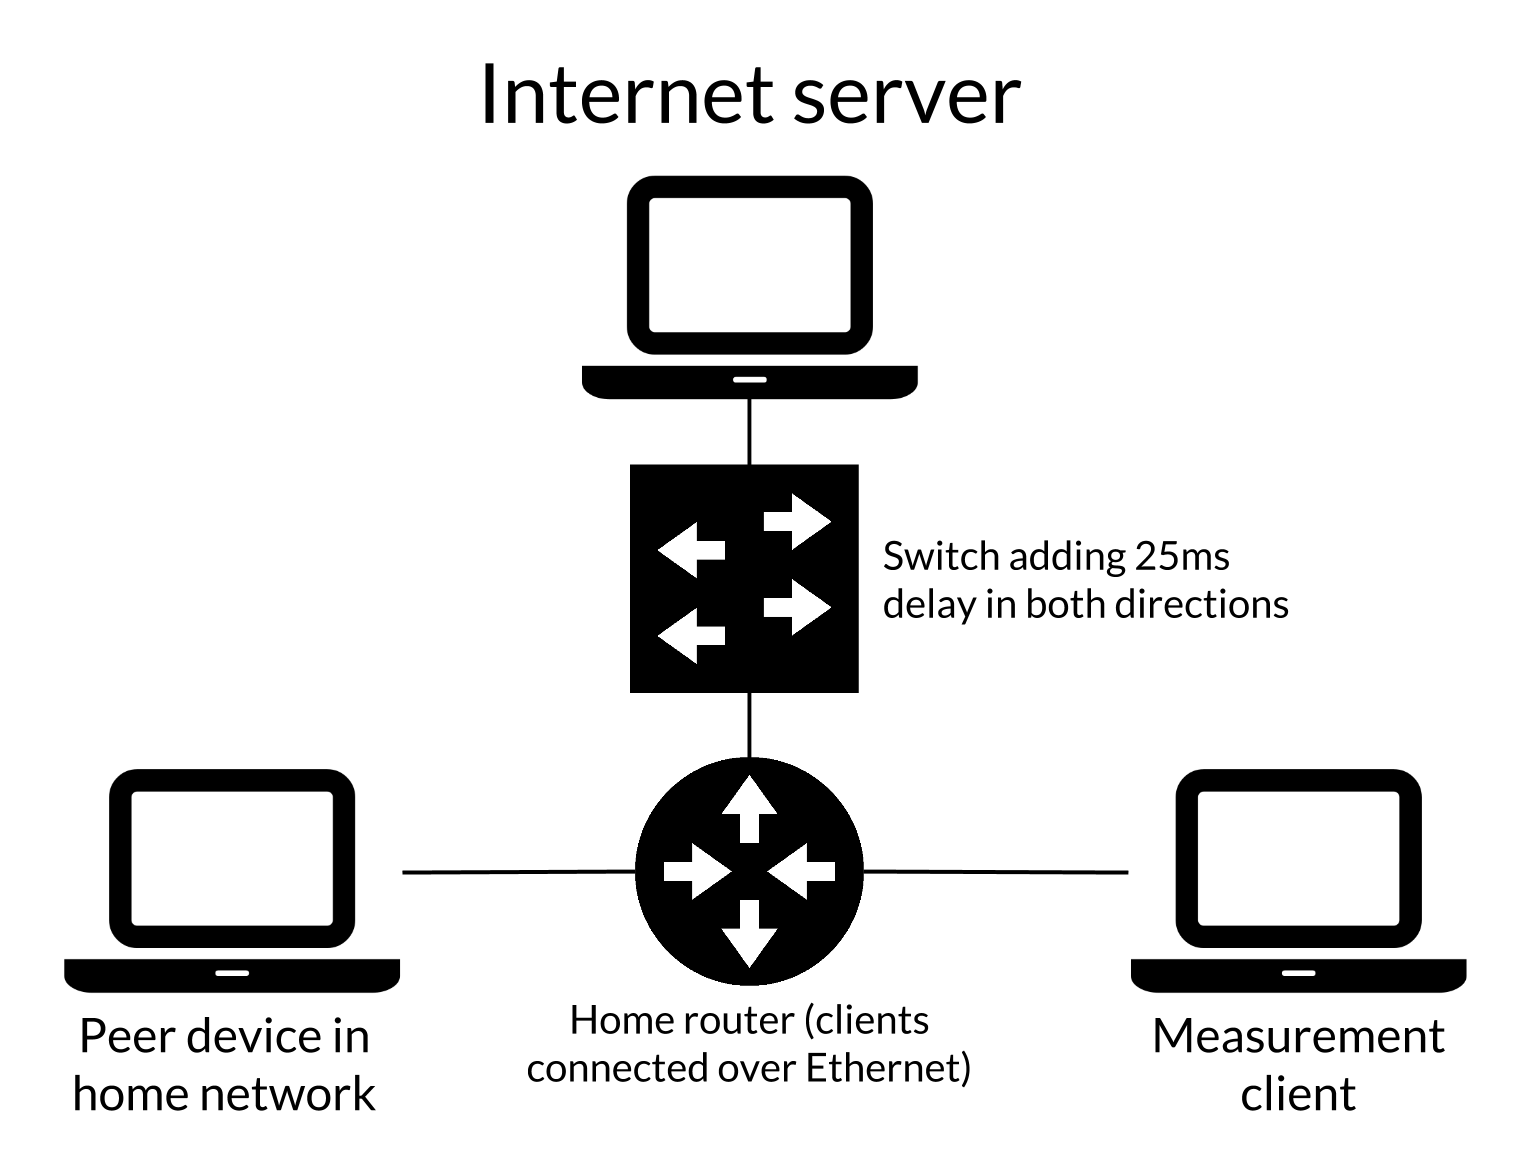
\includegraphics[width=0.65\columnwidth]{figures/setup}
\end{center}
\caption{The testbed setup.}\label{fig:setup}
\end{figure}

Figure~\ref{fig:setup} overviews our testbed. 
The measurement client is a PC running Ubuntu 14.04, OS X El Capitan or Windows 10 with Google Chrome 50 or Mozilla Firefox 45. 
%We test various operating systems and browsers as the implementations of various protocols and the javascript environment are expected to vary from browser to browser. 
Internet Explorer and Safari are excluded due to lack of WebRTC DataChannel support and Opera due to its marginal popularity. 

The measurement client is connected over 100~Mbit/s ethernet to the home router which is a NETGEAR WNDR3700v2 running OpenWRT 15.05. The peer device in the local network is Google Chrome 50 on OS X with 100~Mbit/s ethernet connection to the home router. Finally, the setup has a single controlled Internet server which is a OS X computer connected to the home router over 100~Mbit/s ethernet. To emulate a wide-area link, we place another NETGEAR device acting as a switch between the Internet server and the home router, and use \texttt{netem} to introduce a fixed 25ms delay in both directions (creating an RTT of 50ms between the home router and the Internet server).

\begin{table}[tb]
\label{tab:targets}
\centering
\begin{small}
\begin{tabular}{l l l}
\toprule
\textbf{Target} & \textbf{Technique} & \textbf{Coop.} \\
\midrule
Server & WebRTC DataChannel & yes \\
            & WebSocket & yes  \\
	    & AJAX (GET, POST, HEAD) & yes \\
	    & AJAX (GET, POST, HEAD) & no \\
\midrule
Peer device & WebRTC DataChannel & yes \\
\midrule
Router & AJAX (GET, POST, HEAD) & no \\
\bottomrule
\end{tabular}
\end{small}
\caption {Measurement methods per target.} 
\label{tab:targets}
\end{table}

We have different RTT measurement methods available per target as we summarize in~\autoref{tab:targets}. 
%We test all the available methods to measure the delays to a cooperating Internet server. 
The Internet server runs Apache as a web server and it serves a small one-word document to all the HTTP-based measurement methods. Similarly, we implement a minimal WebSocket server on top of node.js~\cite{socketio} and use Google Chrome for the WebRTC based experiments. 
%We also test the non-cooperative AJAX methods against the Internet server.
Inside the local network we experiment with WebRTC between the measurement client and the peer device, and the non-cooperative AJAX methods to probe the home router. Note that we could use the non-cooperative AJAX methods to probe any device in the local network, but due to similar rounds-trip-times both to the router and the peer device, we do not repeat the AJAX measurements to the peer device. We did also consider the cooperative router case for AJAX but as we will see in the following sections the non-cooperative AJAX methods offer superior performance. % compared to the cooperative case.

\begin{table}[tb]
\label{tab:ping_range}
\centering
\begin{small}
\begin{tabular}{llll}
\toprule
OS & Router & Other device & Server \\
\midrule
OS X & {[$0.2$, $0.4$, $0.9$]} & {[$0.3$, $0.6$, $1.0$]} & {[$50.4$, $50.8$, $52.6$]}\\
Ubuntu & {[$0.2$, $0.2$, $0.4$]} & {[$0.3$, $0.6$, $2.1$]} & {[$50.2$, $50.5$, $51.3$]}\\
Win. & {[$0.3$, $0.8$, $1.2$]} & {[$0.5$, $0.9$, $1.4$]} & {[$50.5$, $51.2$, $51.7$]}\\
\bottomrule
\end{tabular}
\end{small}
\caption {Range [min, median, max] of ICMP ping delays (in ms) for each OS in ms.} 
\label{tab:ping_range}
\end{table}

The experiments are executed as follows. Each client (OS + browser, six combinations) executes the measurements in rounds where we perform an RTT measurement using each available method to the three targets (24 method + target combinations in total). We repeat each measurement round 50 times. At the same time of each measurement, we also execute ICMP ping which serve as a baseline. We use the native ping utility on OS X and Linux. However, because Windows' native ping only has millisecond accuracy, we used True Ping~\cite{tping_windows} on Windows. The baseline RTTs are stable and in expected ranges as we show in Table~\ref{tab:ping_range}.

In the basic experiments we only have a single tab open with a simple empty web page and the embedded javascript code for the measurements. We also test the delay measurements under passive browsing load by opening the 10 most popular web sites in France according to the Alexa ranking~\cite{alexa_top_france} in background tabs. Our results show that adding load adds 
variation to the distributions of measurement overhead, but doesn't impact the conclusions, so we omit them from this paper.

%\begin{table*}[t]
%\centering
%\begin{tabular}{lllll}
%\toprule
%\textbf{Target} & \textbf{Technique} & \textbf{Specifics} & \textbf{Coop.} & \textbf{Comments} \\
%\midrule
%Router & AJAX (GET, POST, HEAD) & :80/ & no & to router's Web-Interface on port 80 \\
%& AJAX (GET, POST, HEAD) & :80/inexistentPath/ & no & provoking 404\\
%& AJAX (GET, POST, HEAD) & to port 80 :1337/ & no & provoking `connection refused'\\
%\midrule
%Other device & WebRTC & Data Channel & yes & Google Chrome as the other endpoint\\
%\midrule
%Server & WebRTC & Data Channel & yes & Google Chrome as the other endpoint\\
%& WebSocket & & yes & \\
%& AJAX (GET, POST, HEAD) & :80/ & yes & cross domain request allowed \\
%& AJAX (GET, POST, HEAD) & :80/ & no & cross domain request forbidden \\
%& AJAX (GET, POST, HEAD) & :80/inexistentPath/ & no & provoking 404 \\
%& AJAX (GET, POST, HEAD) & :1337/ & no & provoking `connection refused' \\
%\bottomrule
%\end{tabular}
%\caption {Measurement methods and targets. Considering all targets, there are 24 different measurement methods in total.} \label{tab:methods}
%\end{table*}
%
%%\begin{table*}[!h]
%%\caption {Example of the randomized order in which measurements are performed. Each measurement run consists of a total of 24 measurements. Each measurement is performed two times and the first result is discarded.} \label{tab:measurement_order}
%%\vspace{0.2cm}
%%\centering
%%\begin{tabular}{lllllllllllllll}
%%\toprule
%%\multicolumn{7}{l}{Measurement run 1} & \multicolumn{7}{l}{Measurement run 2} & ... \\
%%\cmidrule(lr){1-7}
%%\cmidrule(lr){8-14}
%%\cmidrule(lr){15-15}
%%\multicolumn{2}{l}{Method 2} & \multicolumn{2}{l}{Method 20} & \multicolumn{2}{l}{Method 15} & ... & \multicolumn{2}{l}{Method 21} & \multicolumn{2}{l}{Method 18} & \multicolumn{2}{l}{Method 1} & ... \\
%%1 & 2 & 1 & 2 & 1 & 2 && 1 & 2 & 1 & 2 & 1 & 2  \\
%%%WebRTC ping to other machine & Ajax HEAD request to port 1337 of the router & ... & WebSocket ping to Internet Server & Ajax POST request to router on port 80 &\\
%%\bottomrule
%%\end{tabular}
%%\end{table*}
%
%The aim of our experiment is to provide a comprehensive comparison of the accuracy of various web technologies in measuring delay, measured from different OS and Web Browsers to have representative results. Thus our experiment was run on \textit{Microsoft Windows 10}, \textit{Ubuntu Linux 14.04} and \textit{OS X El Capitan}, on each system using the browsers \textit{Google Chrome 50} and \textit{Mozilla Firefox 45}, as these are currently the only ones that support the WebRTC Data Channel, which is used as one of our measurement methods. 
%
%Besides having many different OS and browsers combinations we also performed measurements to various targets: \begin{enumerate*}[label=\alph*)]
%\item a home router
%\item a (simulated) server in the Internet
%\item another device in the same home network.
%\end{enumerate*}
%To each of these targets different measurement methods were utilized, depending on the capabilities of the target platform. 
%For example, it is possible to measure RTTs with WebRTC between two end devices or between one end device and a cooperating Internet server, however, due to the limited capabilities of a commodity home router, it is not possible to use WebRTC in this case. Furthermore, different measurement methods were used depending on whether a target cooperates with the measurements or not. For instance, we assumed that all end devices in a household cooperate because the user has direct control over them. We also suppose to have control over an Internet server, however, we also make measurements to uncooperative servers. On the other hand, we do not expect to have control over the home router, as this would require installing software on it which is not practicable for most users. For all three targets combined, a total of 24 different measurement methods were utilized (\autoref{tab:methods}). 
%The measurement methods were run with an interval of 1~s between each other in a randomized order (\autoref{tab:measurement_order}). Running all 24 measurement methods corresponds to one measurement run. A total of 100 measurement runs were executed for each OS and browser combination, once with load and once without load. For each measurement method and each experiment configuration, 100 delay measurements were obtained.

%The testbed (\autoref{fig:setup}) consisted of the machine under test, which executed the measurements (a device running either Ubuntu, OS X or Windows), a machine which controlled the experiment and collected the data (running OS X) using a node.js program. There was also a third computer (also running OS X) which acted as a server in the Internet. 
%The remote server ran \textit{Apache} for all HTTP-based measurement methods, a minimal \textit{node.js} echo server for the WebSocket ping, based on the WebSocket implementation \textit{WS} and ran Google Chrome for the WebRTC based experiments.
%These three devices were all connected to a home router (\textit{NETGEAR WNDR3700v2} running \textit{OpenWRT 15.05}) using 100~Mbit/s Ethernet. Between the server and the router there was a switch which introduced a constant delay of 25~ms is both directions. 
%
%For each measurement that we performed, we also ran an ICMP ping at the same time, which serves as ground truth. We used the native ping utility on OS X and Linux, however, because Windows' native ping only has millisecond accuracy, we used \textit{True Ping} \cite{tping_windows} on this platform. 
%
%\begin{figure}[h]
%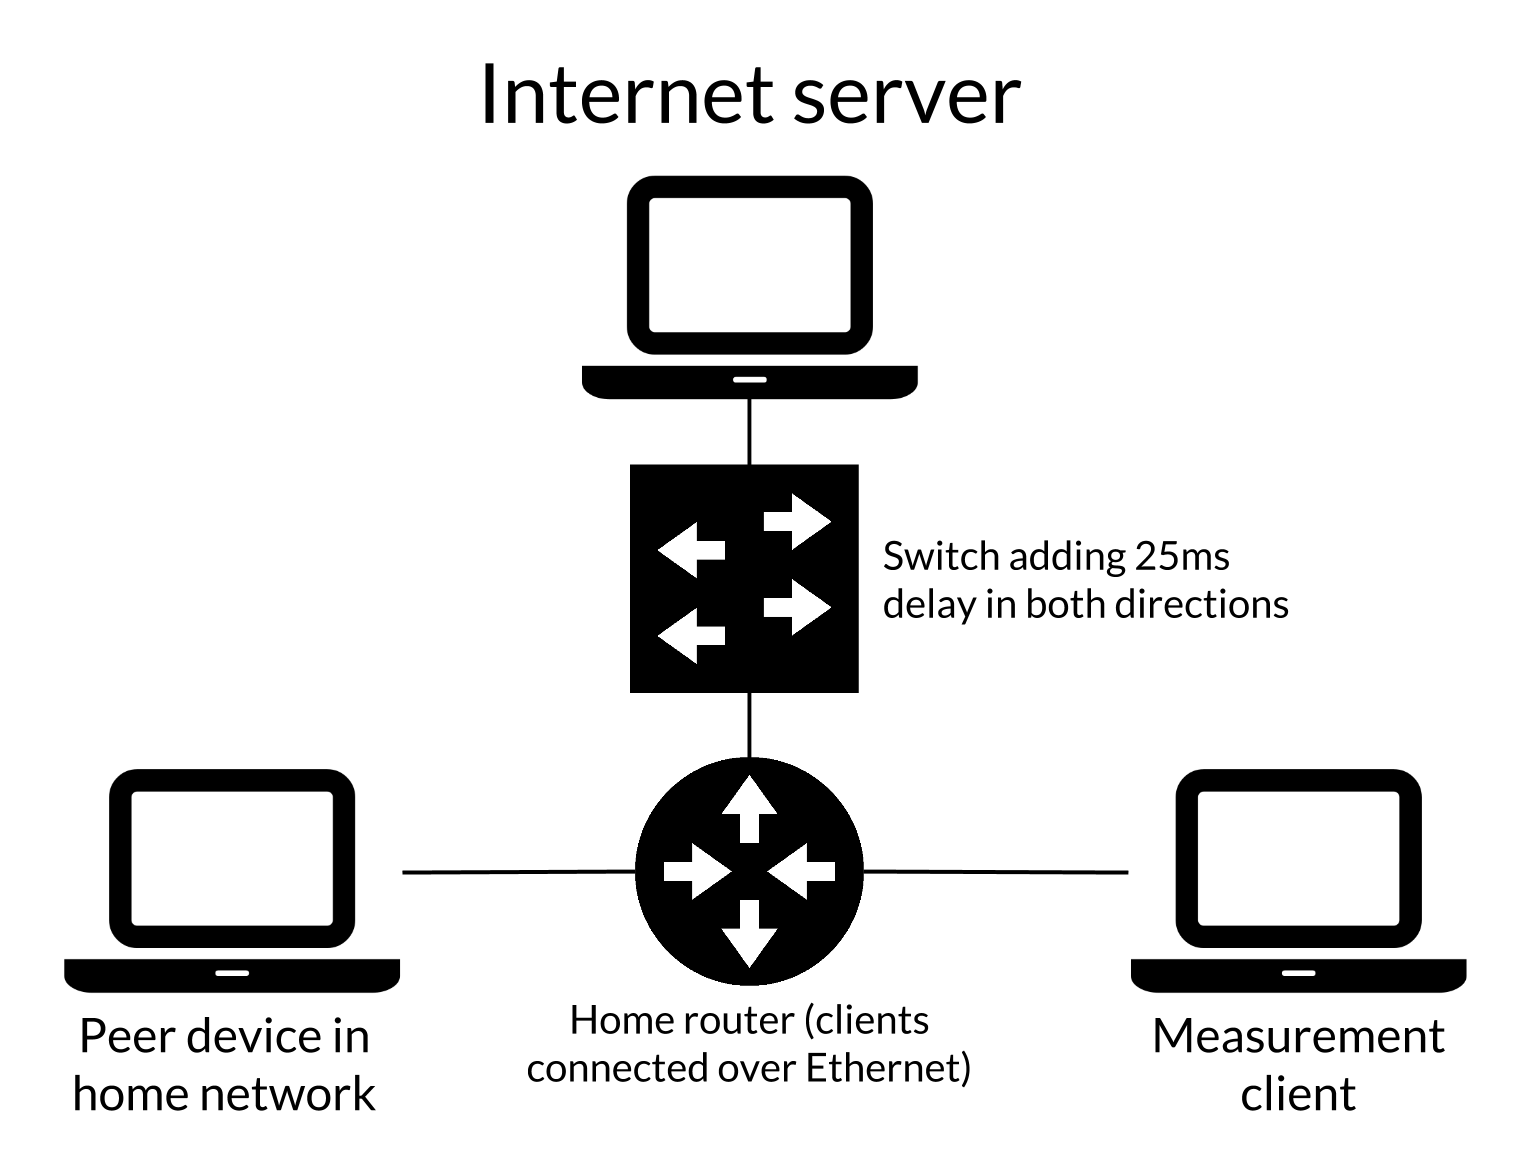
\includegraphics[width=\columnwidth]{figures/setup}
%\caption{The experiment using one device to control the experiment, another one to execute the measurements, a home router, a server and a switch introducing 50 ms RTT to the server.}
%\label{fig:setup}
%\end{figure}
%
%The testbed had stable connectivity and delays throughout all measurements (\autoref{tab:ping_range}). 
%
%\begin{table}[h]
%\caption {Range of ICMP ping during the whole experiment duration for each OS in ms. The left value is the minimum and the right one the maximum.} \label{tab:ping_range}
%\vspace{0.2cm}
%\centering
%\begin{tabular}{rlll}
%\toprule
%OS & Router & Other device & Server \\
%\midrule
%OS X & {[$0.2$, $0.7$]} & {[$0.2$, $1.0$]} & {[$50.3$, $51.7$]}\\
%Ubuntu & {[$0.1$, $0.4$]} & {[$0.2$, $0.7$]} & {[$50.1$, $50.6$]}\\
%Windows & {[$0.3$, $1.3$]} & {[$0.4$, $1.3$]} & {[$50.5$, $54.0$]}\\
%\bottomrule
%\end{tabular}
%\end{table}

\section{Internet Delays}
\label{sec:servers}

In this section we discuss the performance of the browser based delay measurement methods towards Internet targets. This section is partly a reappraisal of the work by Li et al.~\cite{li:imc2013} with respect to the cooperative AJAX GET and WebSocket methods. We add the analysis of WebRTC, comparison between additional AJAX methods and AJAX based measurements to non-cooperating targets. In addition, all our results are based on the high-resolution time API that was not available at the time of the previous study.

The basic metric we use throughout the section is the \textit{delay overhead} that we define as the difference between the native ICMP ping measurement and the studied delay measurement method performed at the same time. As discussed before, this overhead accounts for the protocol overhead and any additional delays caused by the browser and its javascript engine. In general, we are after method(s) with low and/or constant delay overhead.

\subsection{Cooperating Target}

\begin{figure}[thb]
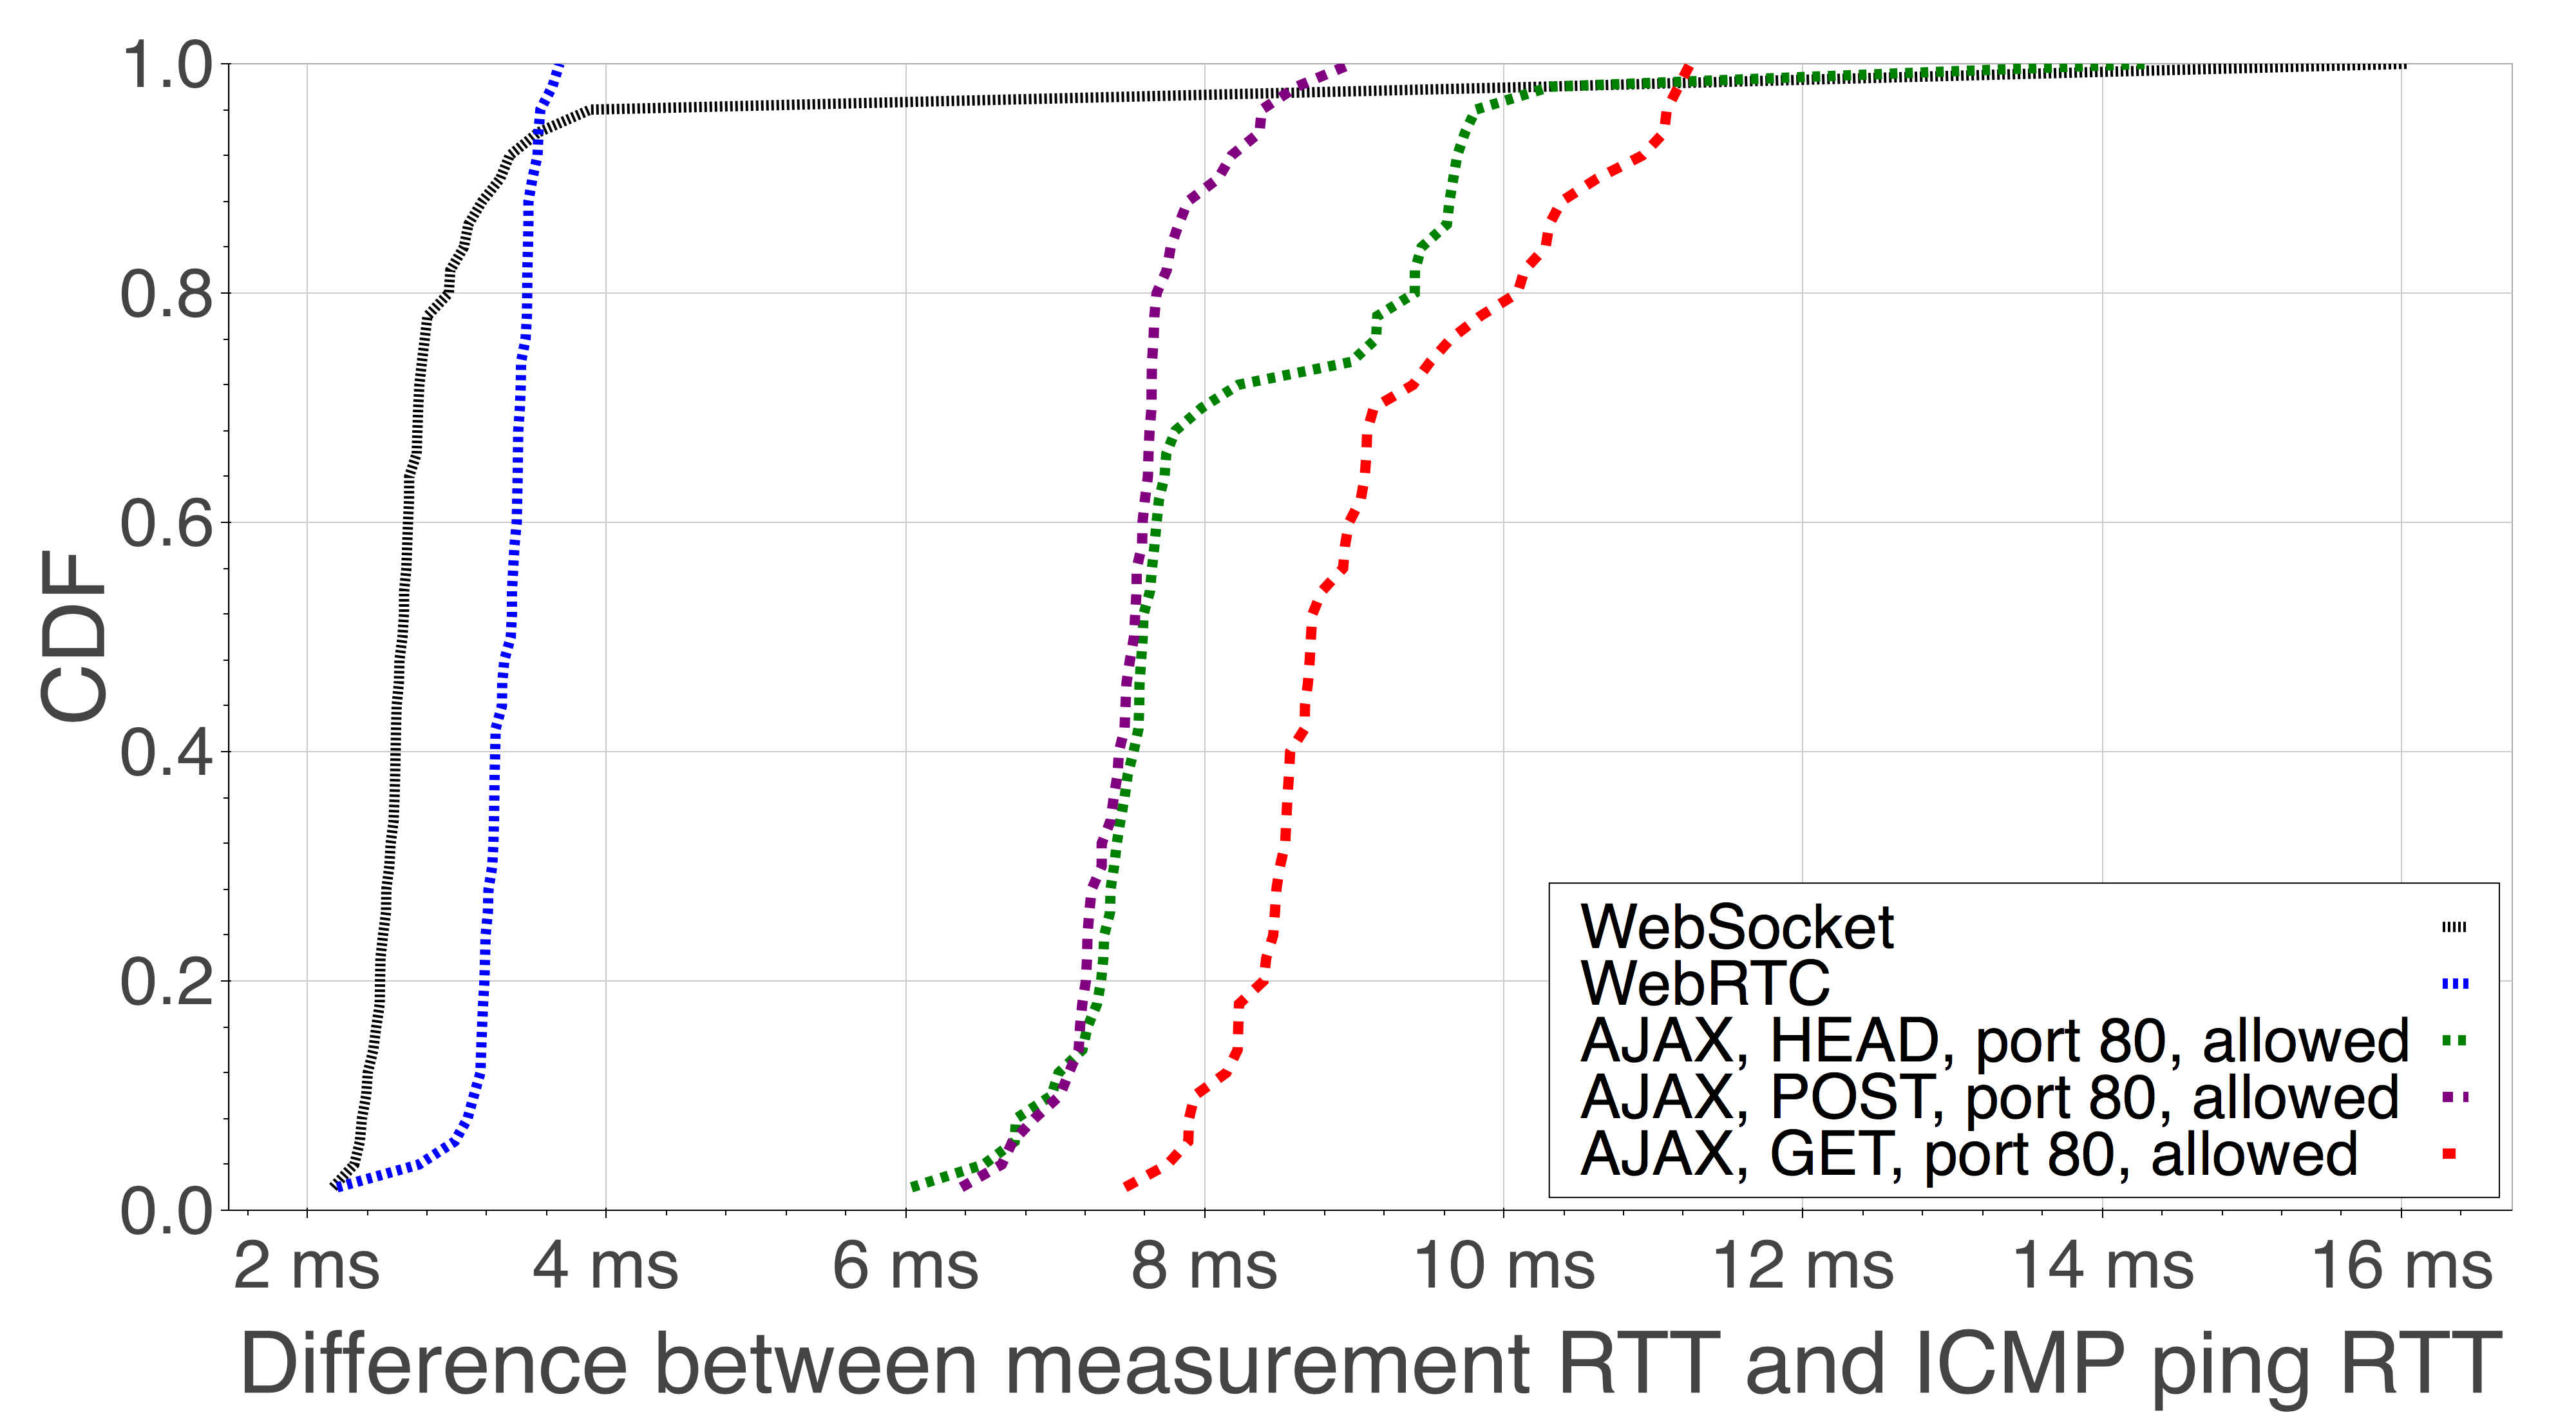
\includegraphics[width=\columnwidth]{figures/inet-coop}
\caption{Delay overheads when measuring a cooperating Internet target (OS X/Chrome).}
\label{fig:inet_coop}
\end{figure}
\vspace{-2mm}

We plot in Figure~\ref{fig:inet_coop} the delay overhead of the various cooperative measurement methods (the depicted results are from OS X with Chrome, the results are similar for Firefox and other operating systems). The WebSocket method results in the lowest overheads, below 3ms, confirming the findings of Li et al.~\cite{li:imc2013}. However, while the WebSocket method generally has a low overhead, we observe a small number of measurements with significantly higher overheads up to 20ms. These occur across all OS and browsers and a further inspection of packet traces reveal that these outliers are not caused by delays in the client browser but rather by a processing delay of up to 20~ms in the WebSocket echo server. These findings are unexpected as our WebSocket server is extremely simple and leverages a widely used library but should be nevertheless taken into account if using WebSockets for delay measurements. Interestingly, the WebRTC method shows rather good and stable performance with only a slightly higher, above 3ms, overhead compared to WebSocket. Moreover, the overhead shows little variance making WebRTC a good candidate for delay measurements with cooperating targets.

The AJAX based methods perform clearly worse due to the HTTP protocol overhead (larger payloads and request + response parsing) and the delay overheads are between 7-9ms in the median case. We compare the HTTP GET, POST and HEAD methods in Figure~\ref{fig:inet_coop}, and observe that POST and HEAD are somewhat better than GET (usually below 8ms overhead compared to more than 8ms), and that POST has additionally lower variance making it the best AJAX based method for delay measurements. 

\subsection{Non-cooperating Target}

\begin{figure}[h]
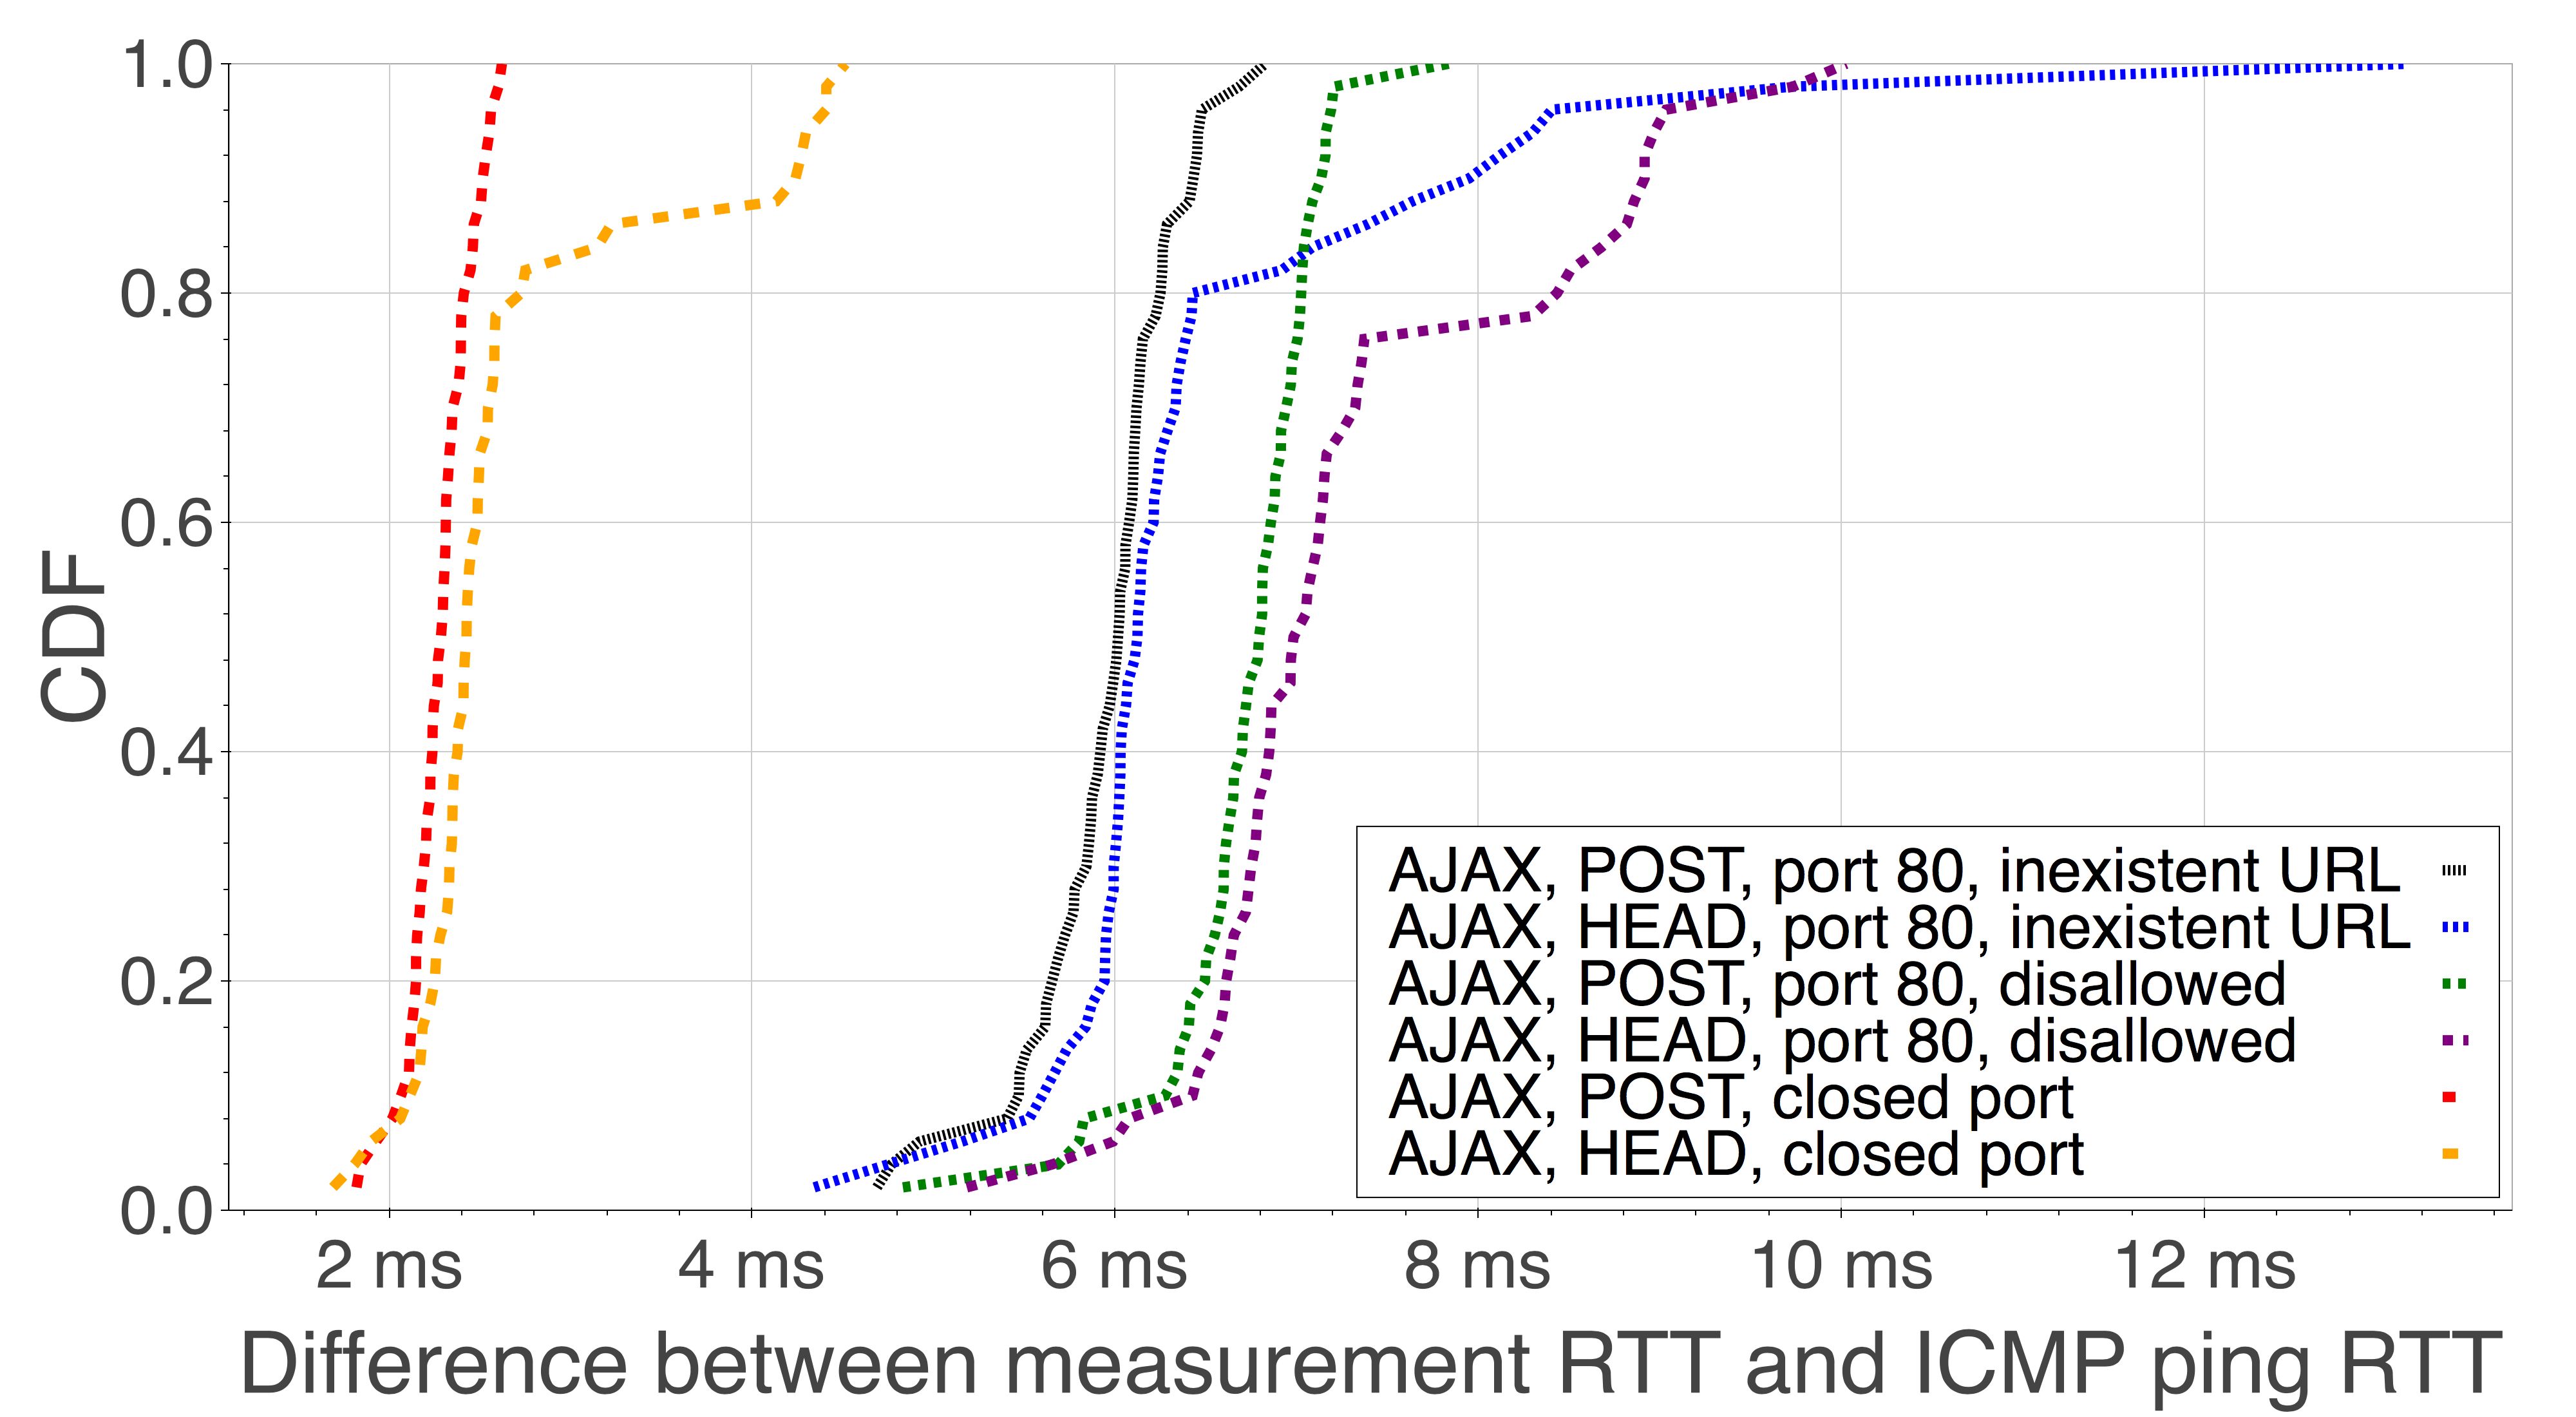
\includegraphics[width=\columnwidth]{figures/inet-non-coop-new}
\caption{Delay overheads to an uncooperative Internet target using AJAX (OS X/Chrome).}
\label{fig:inet_non_coop_new}
\end{figure}
\vspace{-2mm}

In Figure~\ref{fig:inet_non_coop_new} we compare the different non-cooperative AJAX methods (inexisting URL, unallowed cross-origin request and a request to a closed port). We exclude HTTP GET as similarly to the cooperative case it performs generally worse than HEAD and POST. An AJAX request to a closed port shows the lowest overhead of around 2ms and is comparable, or even better in performance than the best cooperating methods (WebSocket and WebRTC). The invalid cross-origin request and access to non-existing resource have similar overhead, the former being slightly worse with around 7ms overhead in general. As in the cooperating server case, the request type has an impact on the overheads: POST has a slightly lower overhead than HEAD and similarly, POST has less variation in its overhead. Note also that the overhead from error response is smaller than the overhead when fetching an existing resource (order of 1ms). These results are similar for Firefox and across the operating systems.


\begin{figure}[h]
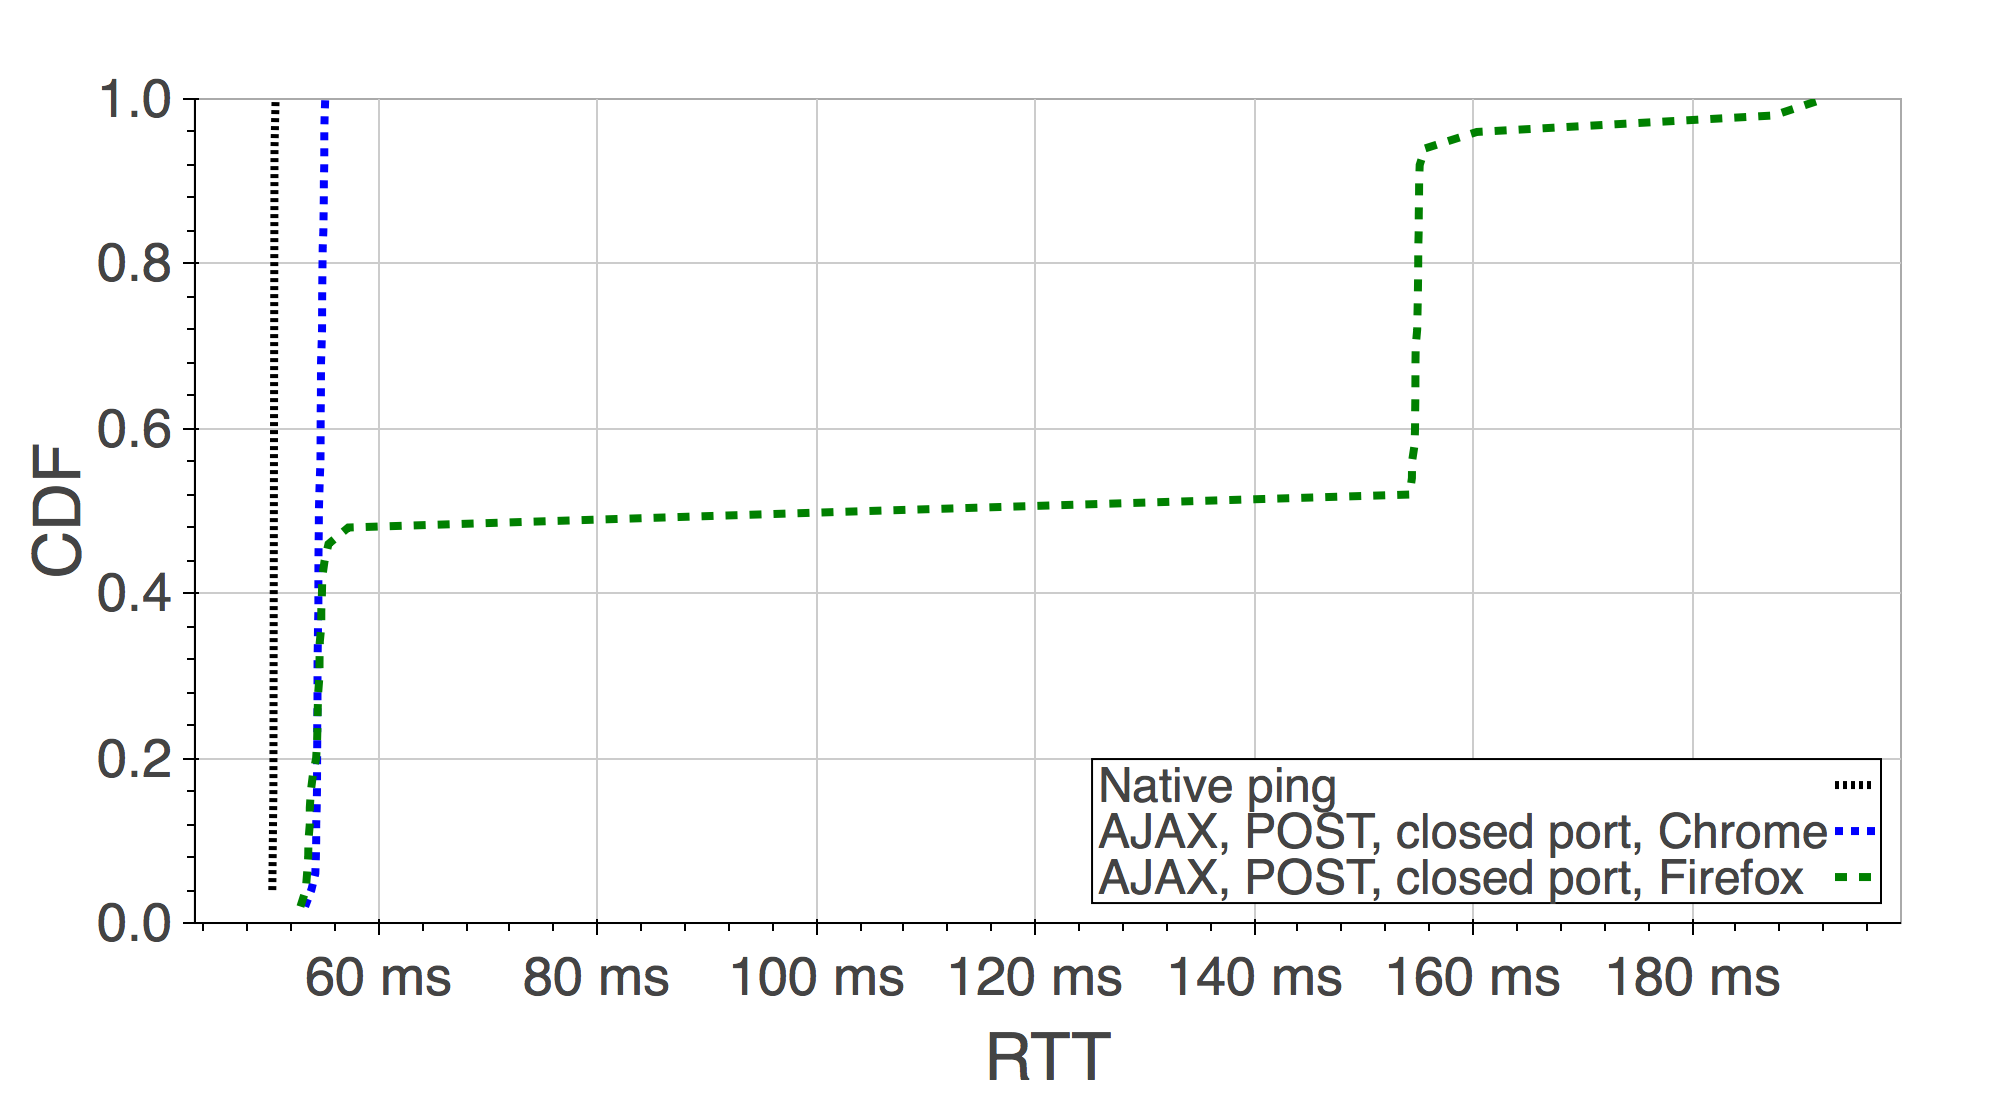
\includegraphics[width=\columnwidth]{figures/inet-comp-chrome-ff}
\caption{Delay overheads to an Internet server on a closed port (Ubuntu/Firefox, Chrome).}
\label{fig:inet_comp_chrome_ff}
\end{figure}
\vspace{-2mm}

The AJAX request to a closed port seems attractive method for delay measurements. However, in practise it may be unusable due to the firewall problems discussed before. Even if the firewalls are not an issue, we observe another problem with the method. Namely, when requesting a page from a closed port on Firefox, the request does not always immediately return an error to our measurement code (\autoref{fig:inet_comp_chrome_ff}). The packet traces reveal that Firefox always tries to establish three TCP connections at the same time and raises the error randomly after it gets the first, second or third connection refused, meaning after one, two or three RTTs. Furthermore, the method of sending AJAX requests to closed ports only works from an OS X or Linux host. Windows never immediately reports the connection refused error to an application upon receiving a RST packet but instead retries several times before quitting the connection attempt~\cite{microsoft_tcp_retries} which makes this method unusable on Windows. 

%\subsection{Influence of Load}
%
%\begin{figure}[thb]
%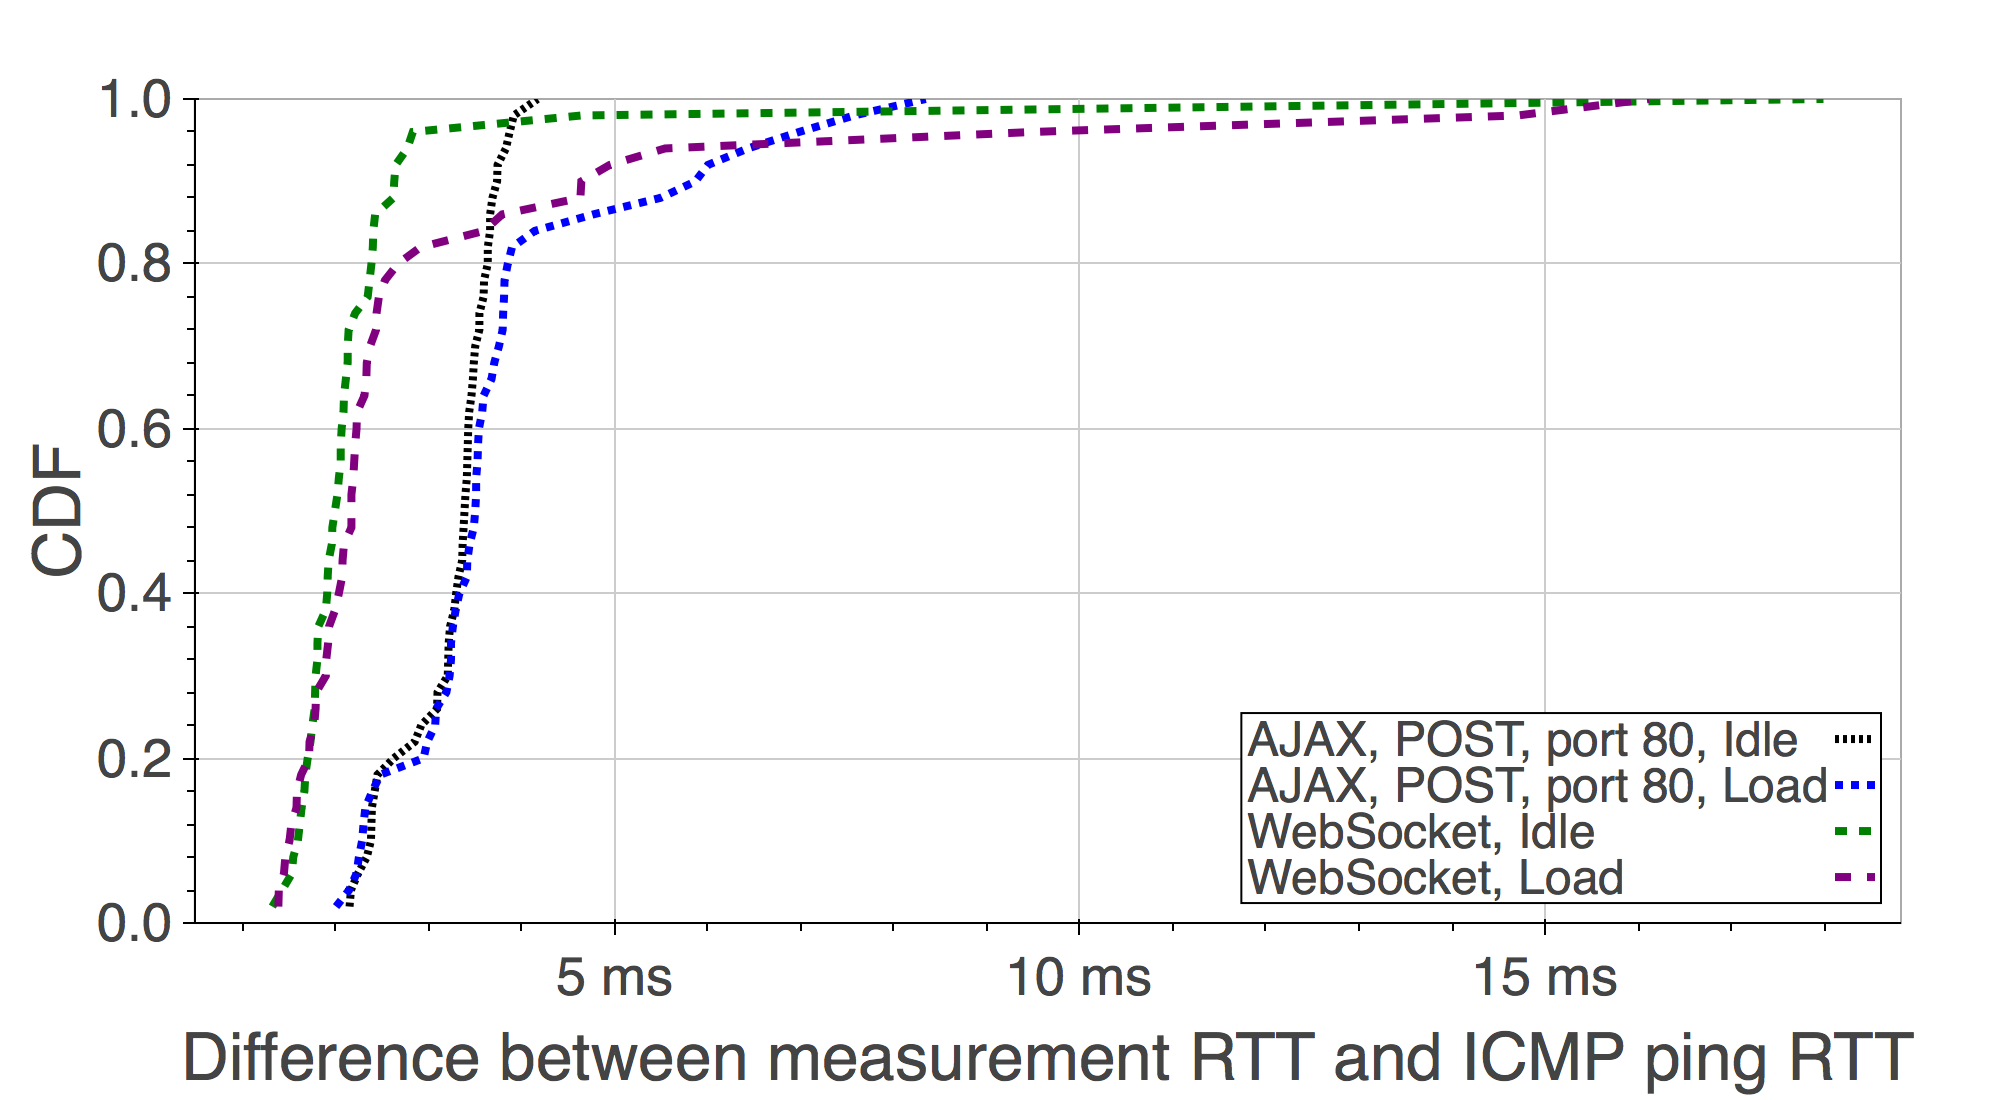
\includegraphics[width=\columnwidth]{figures/inet-comp-load-ff}
%\caption{Delay overhead to an Internet server when being idle or under load (Ubuntu/Firefox).}
%\label{fig:inet_comp_load}
%\end{figure}
%
%Figure~\ref{fig:inet_comp_load} compares the delay overheads of AJAX POST and WebSocket when the measurement client browser is under load or not. In general, the effect of load is higher variability in the overheads, the median cases remain the same. In general, Firefox is more impacted by load than Chrome where load has almost no effect, The results are consistent across all the methods and the three operating systems. We believe this might be caused by the multi-process architecture of Google Chrome~\cite{chrome_multi-process_2008} where each web page runs in an independent process while in Firefox, currently, there is one process for all web pages and for the browser UI~\cite{firefox_multiprocess_2016}.
%
%

\section{Local Network Delays}
\label{sec:local}

In this section we focus on the local network delay measurements. The big challenge in measuring the delays in the local network is the overhead that in many cases is in the same order as the actual network delays.

\begin{figure}[thb]
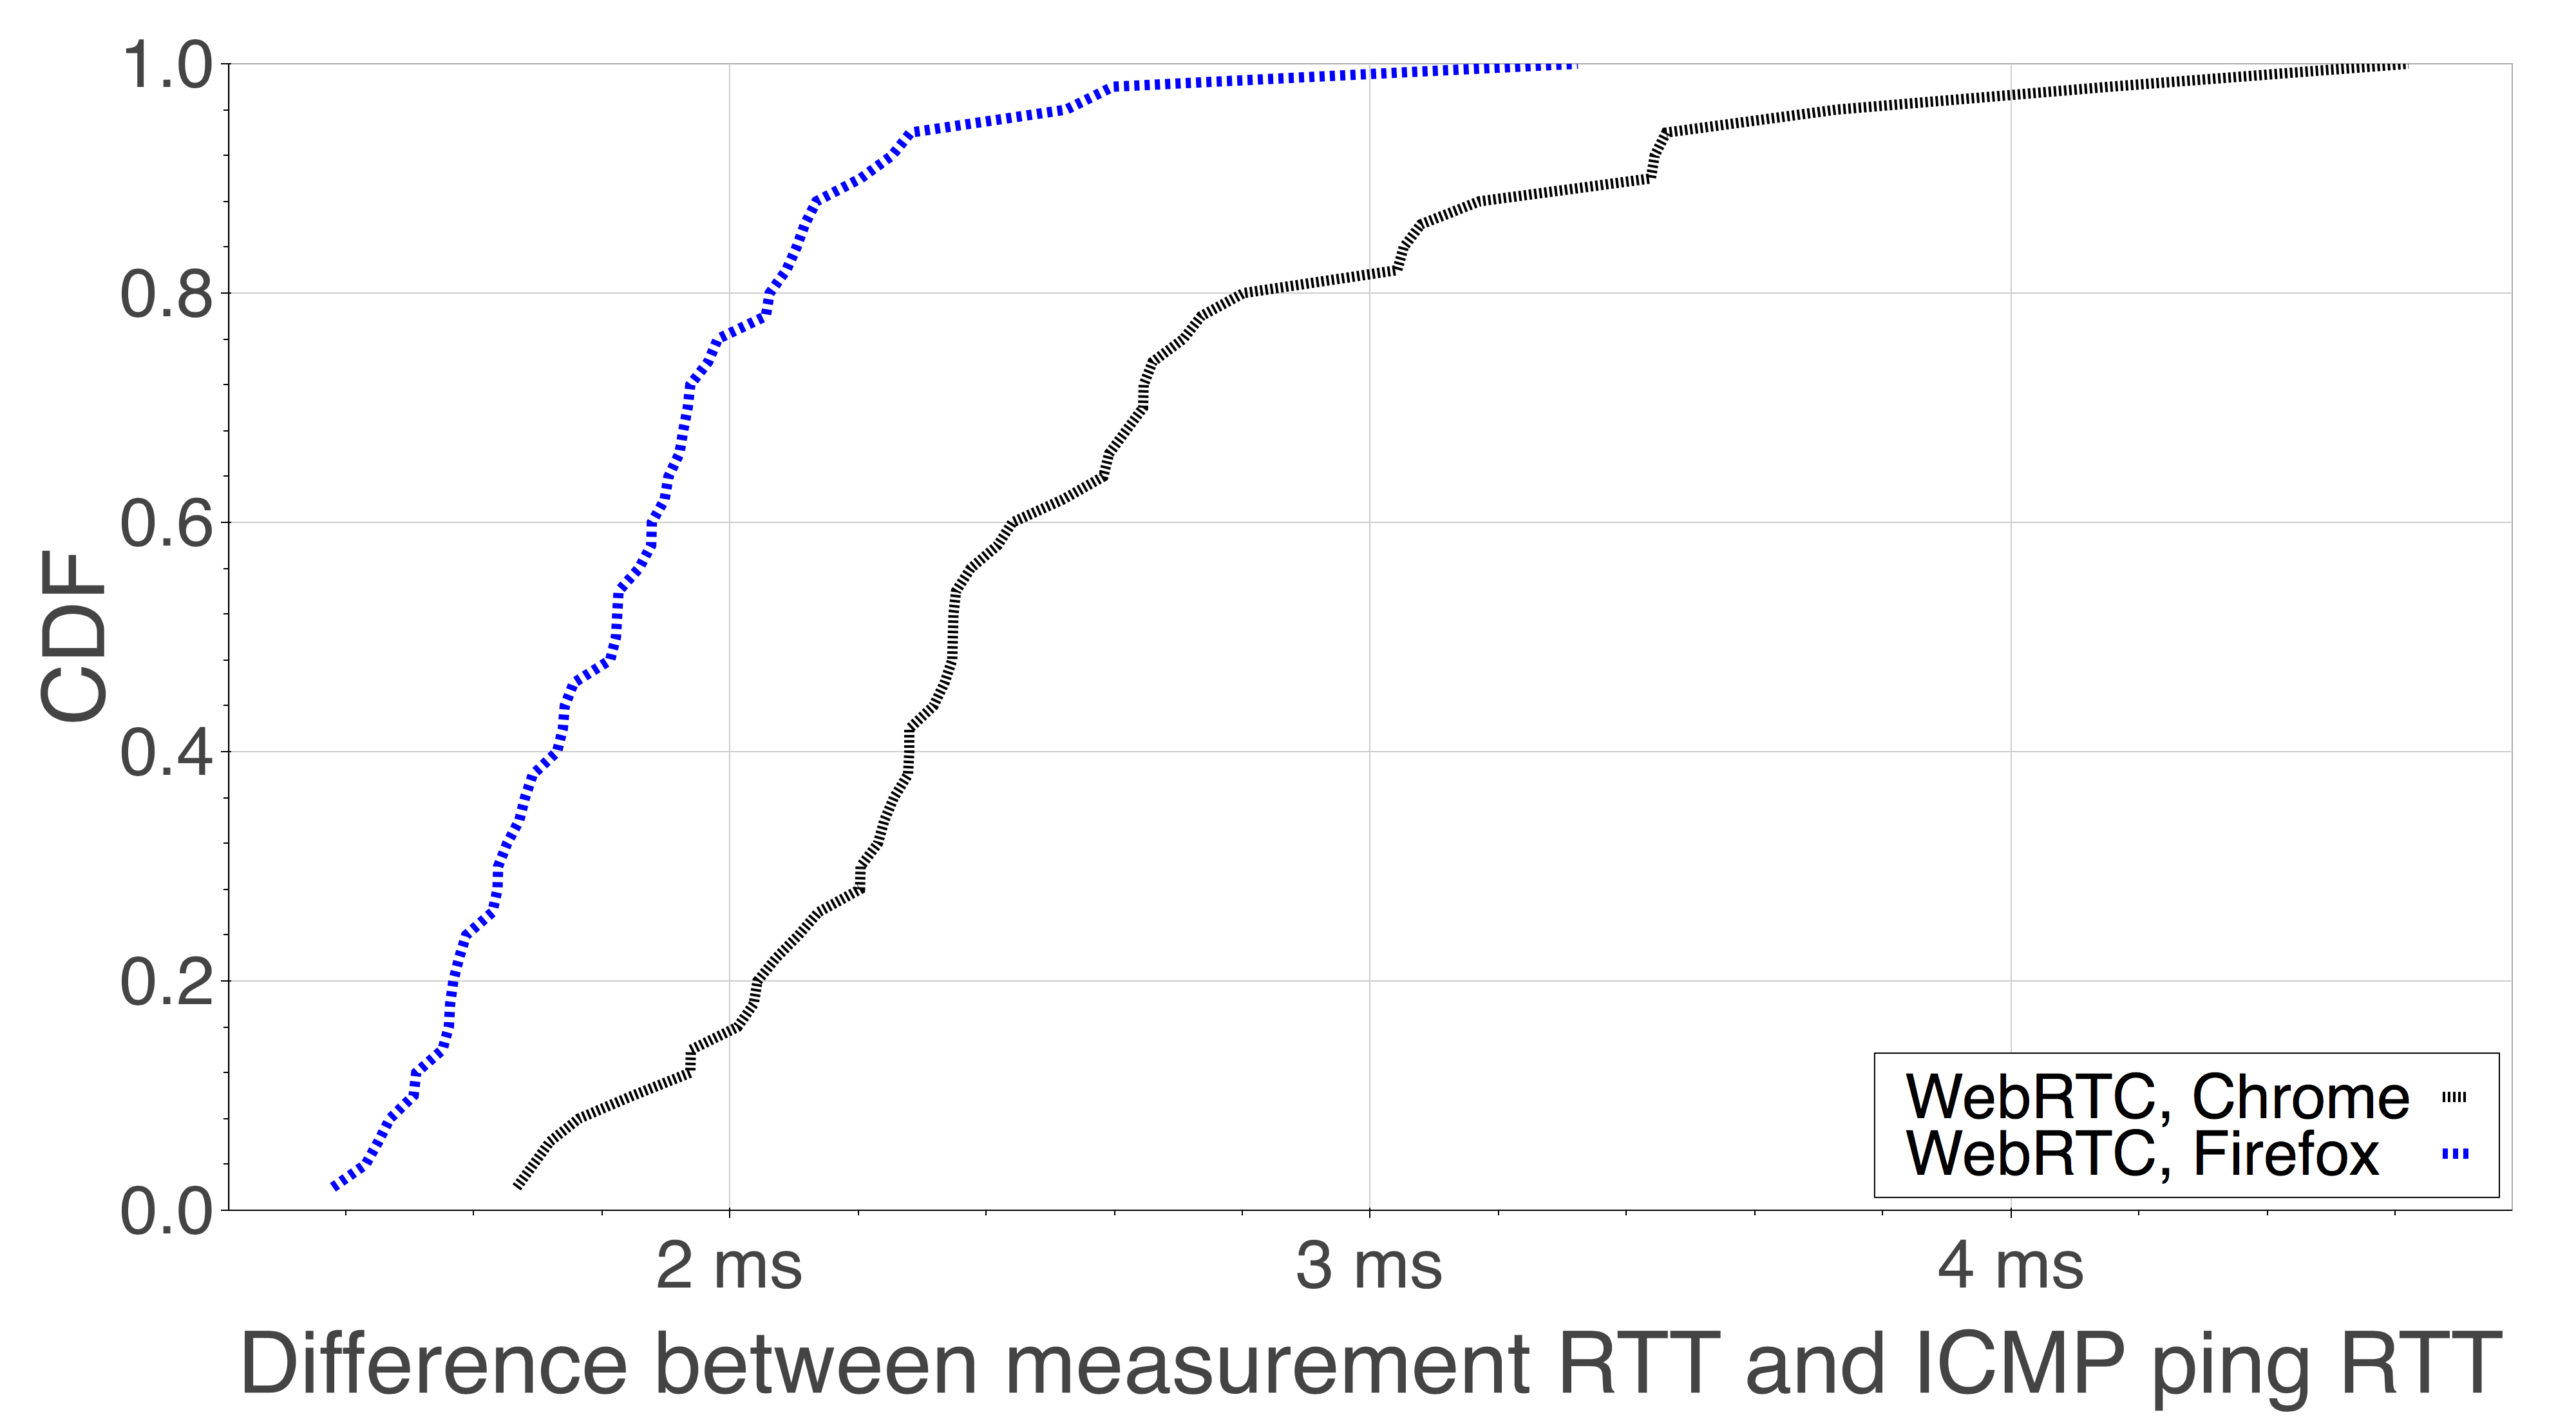
\includegraphics[width=\columnwidth]{figures/other-machine-comp-chrome-ff}
\caption{Delay overheads of WebRTC in local network (OS X/Chrome, Firefox).}
\label{fig:peer_comp_chrome_ff}
\end{figure}
%\vspace{-2mm}

We measure the delays to a peer device in the same local network using WebRTC and the results for OS X are shown in Figure~\ref{fig:peer_comp_chrome_ff}. The delay overhead is similar to the Internet server case discusses earlier, below 3ms for 80\% of the time for Chrome, and below 2ms for 80\% for Firefox. 

\begin{figure}[thb]
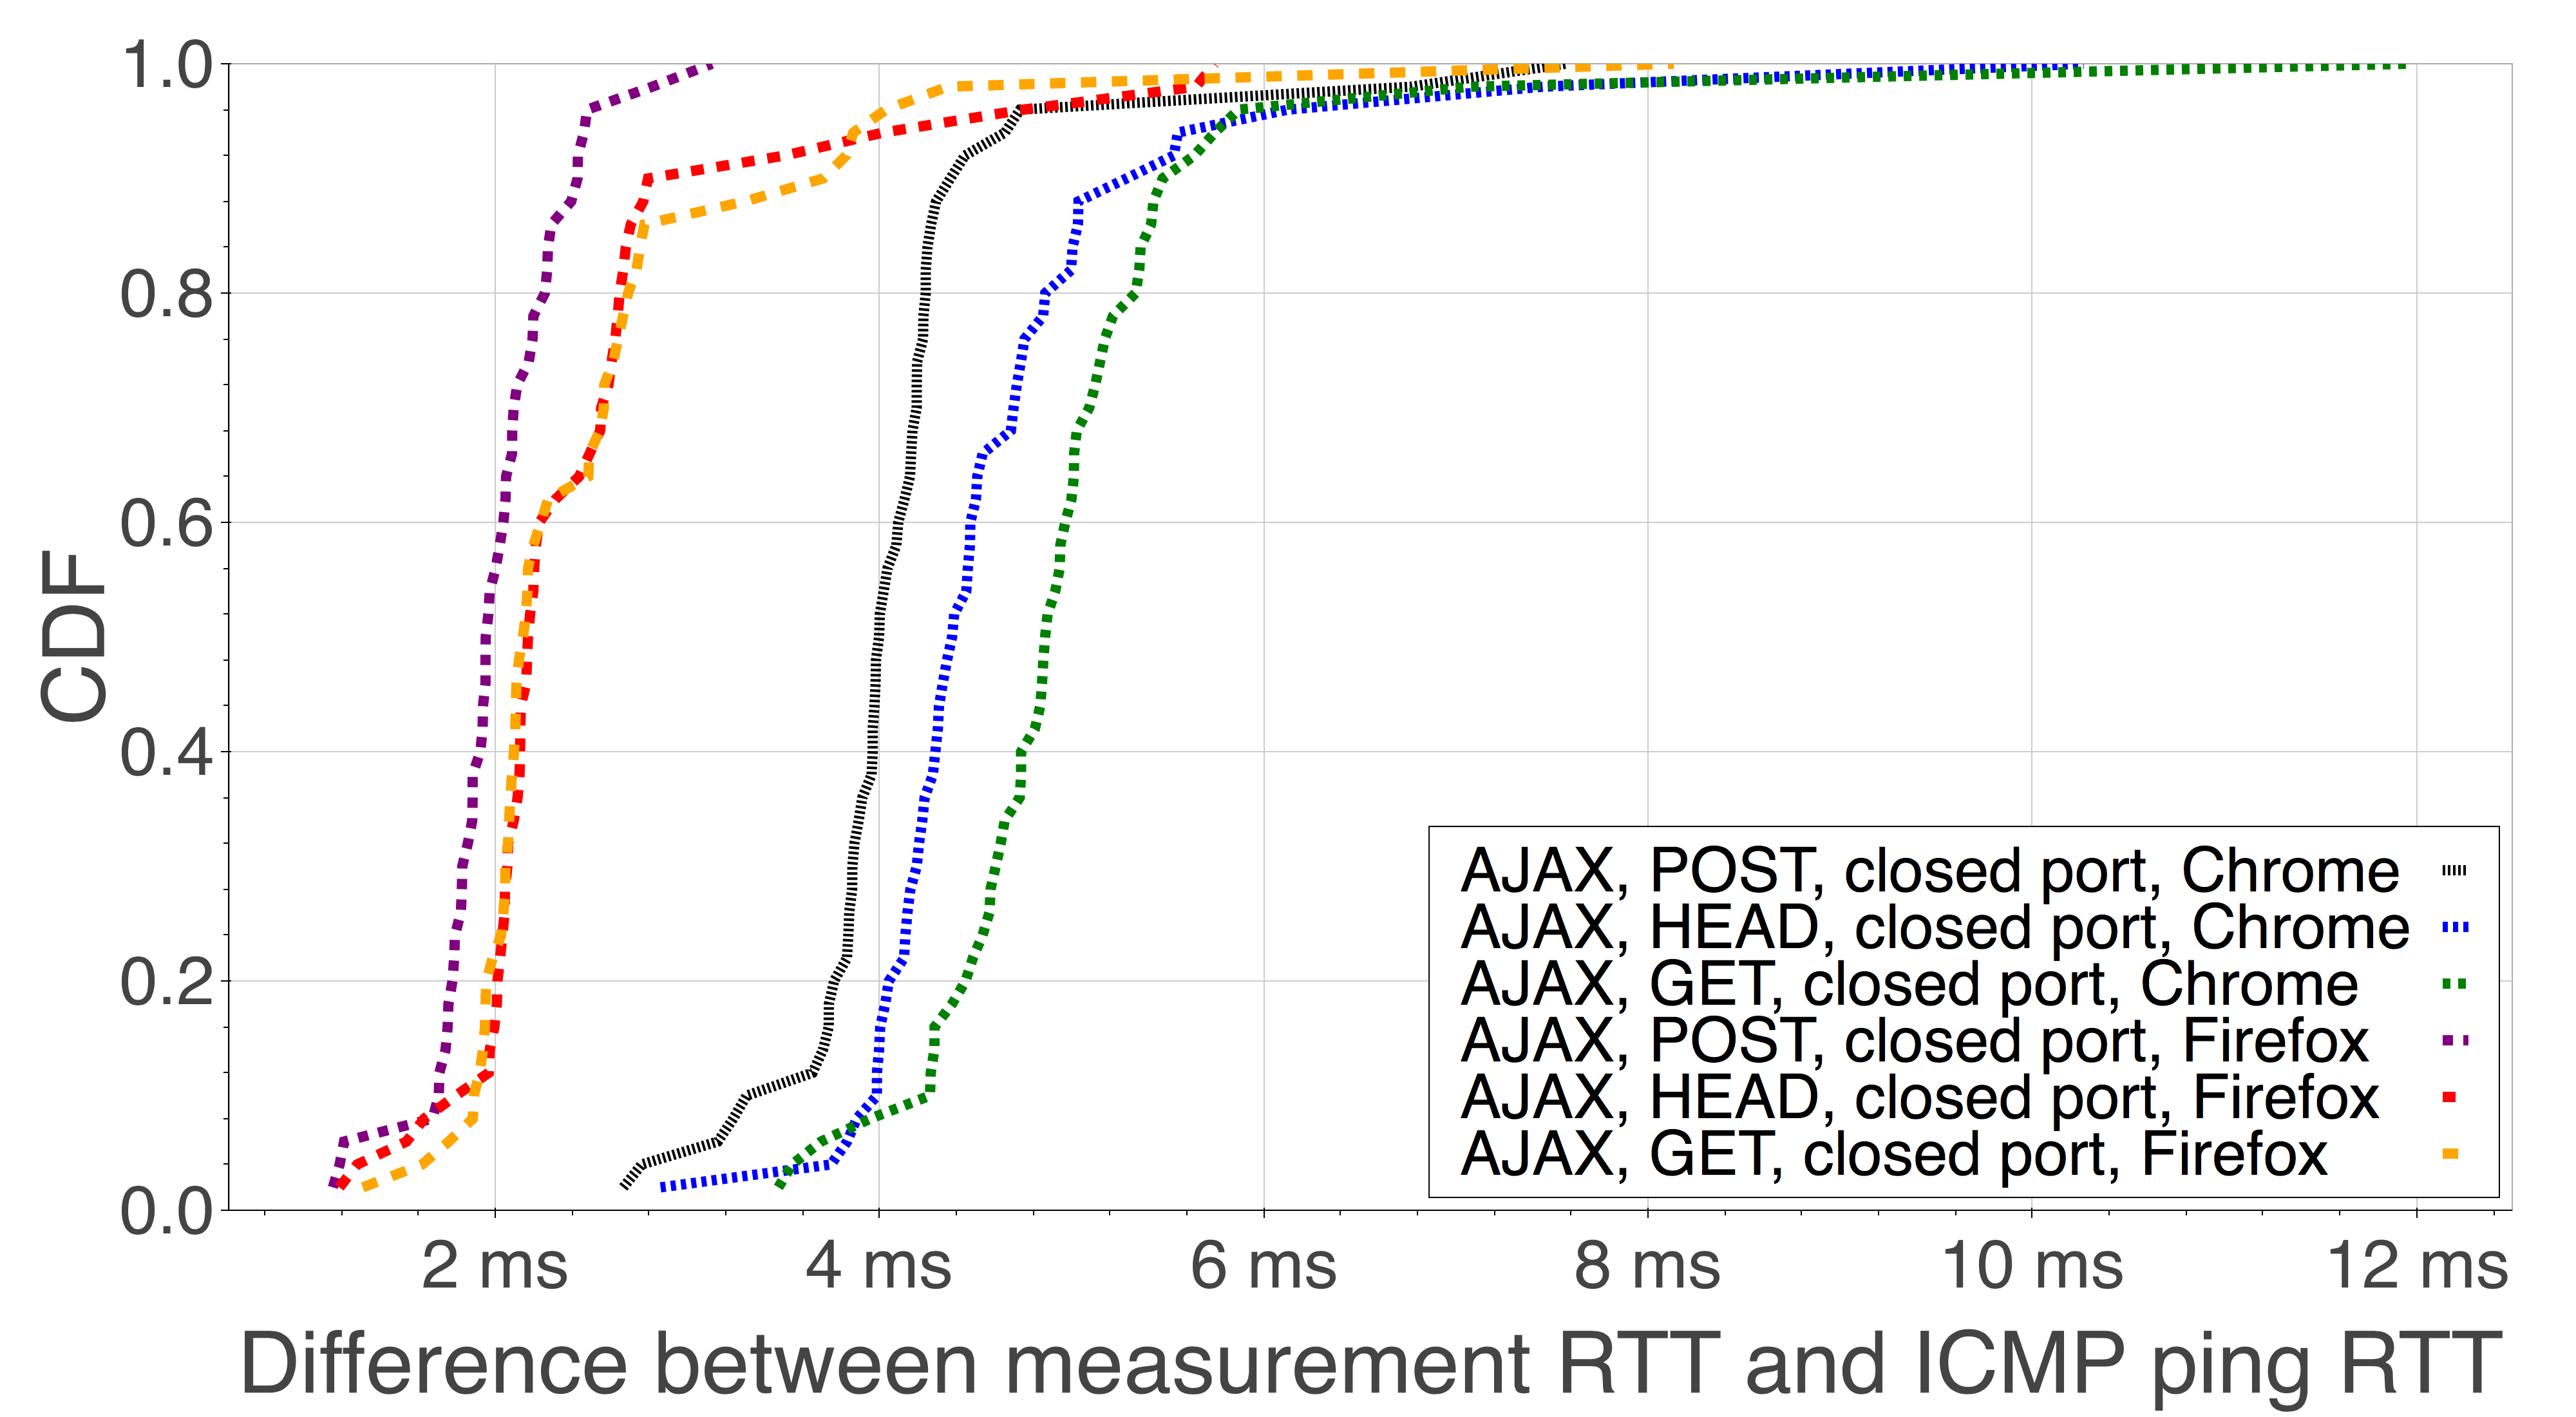
\includegraphics[width=\columnwidth]{figures/router-comp-chrome-ff}
\caption{Delay overheads to a home router (OS X/Chrome, Firefox).}
\label{fig:router_comp_chrome_ff}
\end{figure}
%\vspace{-2mm}

For the home router, we test various AJAX based methods. Figure~\ref{fig:router_comp_chrome_ff} compares the methods with the lowest overhead for Chrome and Firefox which is the various AJAX requests to a closed port (\emph{i.e.} we are basically measuring the TCP handshake delay). There is some variation between the different methods due to browser processing. This difference is particular large for Chrome. In general, the overhead is around 2ms for Firefox, and around 4ms for Chrome. 

Considering that the baseline delay of our local network setup is less than 1ms, the overheads for both peer device and router delay measurements are still high. However, our setup is basically testing the worst case as we connect everything via ethernet. Typical home networks are using mostly wireless connections, and especially in case of trouble, the wireless delays can be in the order of several tens of milliseconds.



%\section{Discussion}
%\label{sec:loca}
%
%
%\begin{table*}[thb]
%\caption {Measurement method with least overhead in milliseconds selected for each OS and browser by median in case of no additional load in the browser. First and third quartile in brackets} \label{comparison}
%\vspace{0.2cm}
%\centering
%\begin{tabular}{ll|ll|ll|ll}
%\noalign{\hrule height 1pt}
%\multirow{2}{*}{OS} & \multirow{2}{*}{Browser} & \multicolumn{2}{l|}{Router} & \multicolumn{2}{l|}{Other machine} & \multicolumn{2}{l}{Server} \\
%%\cline{3-8}
%&& Value & Method & Value & Method & Value & Method\\
%\noalign{\hrule}
%\multirow{2}{*}{OS X} & Chrome & 1.9 [1.8, 2.2] &Ajax Post, closed port & 2.3 [1.7, 3.6] &WebRTC & 2.3 [2.0, 2.6]& WebSocket \\
%& Firefox & 3.1 [2.9, 3.4] &Ajax Get, closed port & 1.8 [1.5, 2.4]& WebRTC & 2.4 [2.0, 3.5]& WebSocket\\
%\noalign{\hrule}
%\multirow{2}{*}{Ubuntu} & Chrome & 4.0 [3.3, 4.7] &Ajax Post, closed port & 2.7 [2.2, 3.1]& WebRTC & 2.8 [2.5, 4.0]& WebSocket\\
%& Firefox & 2.0 [1.4, 2.5]& Ajax Post, closed port & 1.8 [1.5, 2.1]& WebRTC & 2.2 [1.8, 53.7]& Ajax Get \\
%\noalign{\hrule}
%\multirow{2}{*}{Win.} & Chrome & 3.7 [2.3, 4.3]& Ajax Post, inval.~path & 2.1 [1.4, 2.5]& WebRTC & 2.1 [1.6, 4.1]& WebSocket\\
%& Firefox & 3.3 [1.6, 3.7]& Ajax Post, inval.~path & 1.7 [1.0, 2.1]& WebRTC & 2.0 [1.5, 2.8]& WebSocket\\
%\noalign{\hrule height 1pt}
%\end{tabular}
%\end{table*}
%
%\xxx{TODO: discuss the table and recommend best methods for each combi - or remove ?}

%\section{Internet delays}
%\label{sec:servers}
%
%%\xxx{here just focus on the results no more method or setup discussion here. should have been before.}
%%The remote server ran \textit{Apache} as a web server for all HTTP-based measurement methods, a minimal \textit{node.js} echo server for the WebSocket ping, based on the WebSocket implementation \textit{WS} and ran Google Chrome for the WebRTC based experiments.
%
%We used the following three uncooperative methods: \begin{enumerate*}[label=\alph*)]
%\item Ajax requests to port 80 with cross domain requests not being allowed by the server
%\item Ajax requests to an inexistent URL
%\item Ajax requests to a closed port.
%\end{enumerate*}
%Interestingly, when requesting an inexistent page, the RTT depends on the request type that is used, with POST we get the lowest RTTs and with GET the largest (see \autoref{fig:inet_non_coop}). This behavior is consistent across both Google Chrome and Mozilla Firefox and also does not depend on the OS being used.
%
%\begin{figure}[h]
%\label{fig:inet_non_coop}
%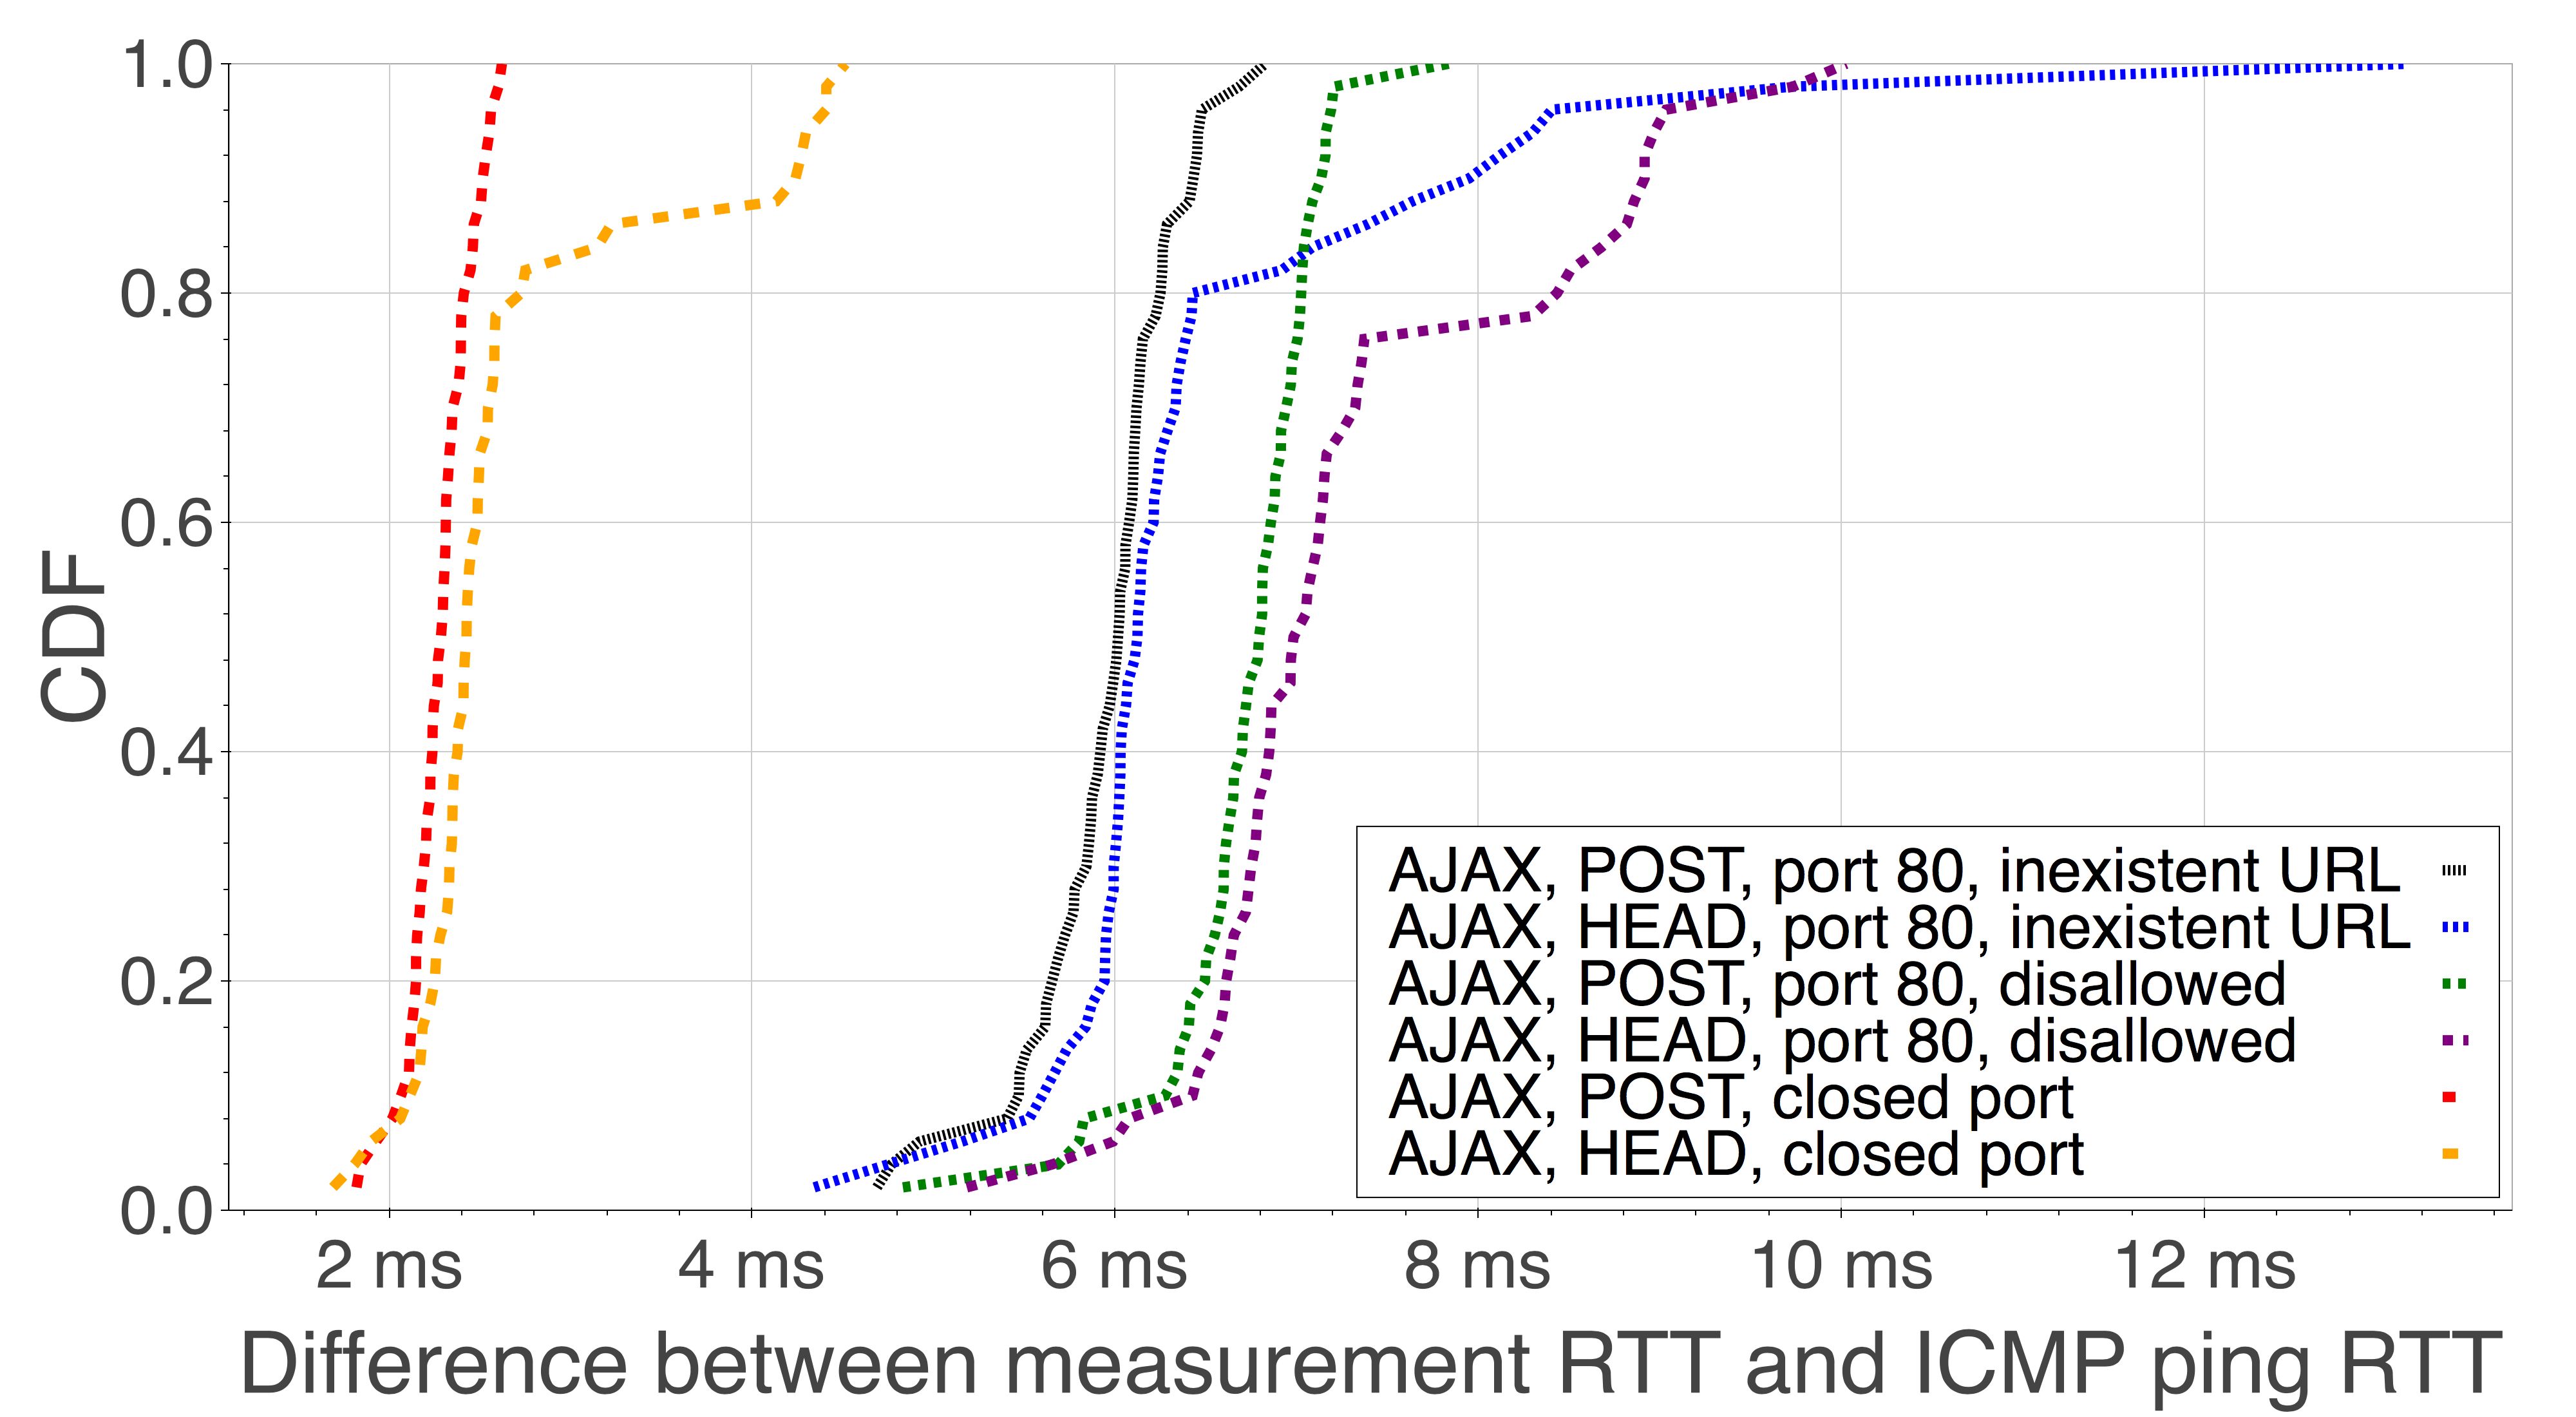
\includegraphics[width=\columnwidth]{figures/inet-non-coop-new}
%\caption{Delay overheads to an uncooperative server in the Internet using either AJAX HEAD or POST on Mac using Chrome.}
%\end{figure}
%
%%\todo[inline]{Is the following section necessary?}
%%Another possibility is to use Ajax requests to a closed port on the router. In this case, the browser sends a SYN packet to the router on an arbitrary closed port to try to establish a TCP connection. Because the port is closed, the router replies with a RST packet, raising the error \textit{connection refused} in the browser. 
%
%When requesting a page from a closed port we see that Mozilla Firefox does not always immediately return an error to our measurement code (\autoref{fig:inet_comp_chrome_ff}). The packet traces reveal that Firefox always tries to establish three TCP connections at the same time and raises the error after it gets the first, second or third connection refused, meaning after one, two or there RTTs. Furthermore, the method of sending AJAX requests to closed ports only works from an OS X or Linux host. Windows does not immediately report \textit{connection refused} to an application upon receiving a RST packet but instead retries several times before quitting the connection attempt \cite{microsoft_tcp_retries}, which leads to unusable delay measurement results (\autoref{tab:weird_win_table}). 
%
%\begin{table}[h]
%\label{tab:weird_win_table}
%\centering
%\begin{tabular}{llll}
%\toprule
%OS & GET & POST & HEAD \\
%\midrule
%Linux & 4.8 & 4.1 & 4.4 \\
%Windows & 1021.2 & 1020.0 & 1021.8 \\
%\bottomrule
%\end{tabular}
%\caption {Delay overheads to an uncooperative server using Ajax in Chrome from Linux and Windows in milliseconds.}
%\end{table}
%
%%However, this method is only of limited utility in the case of Internet servers as many have firewalls which filter and drop packets directed to closed ports. We will, however, use this method to a home router in \S\ref{sec:router}. 
%
%\begin{figure}[h]
%\label{fig:inet_comp_chrome_ff}
%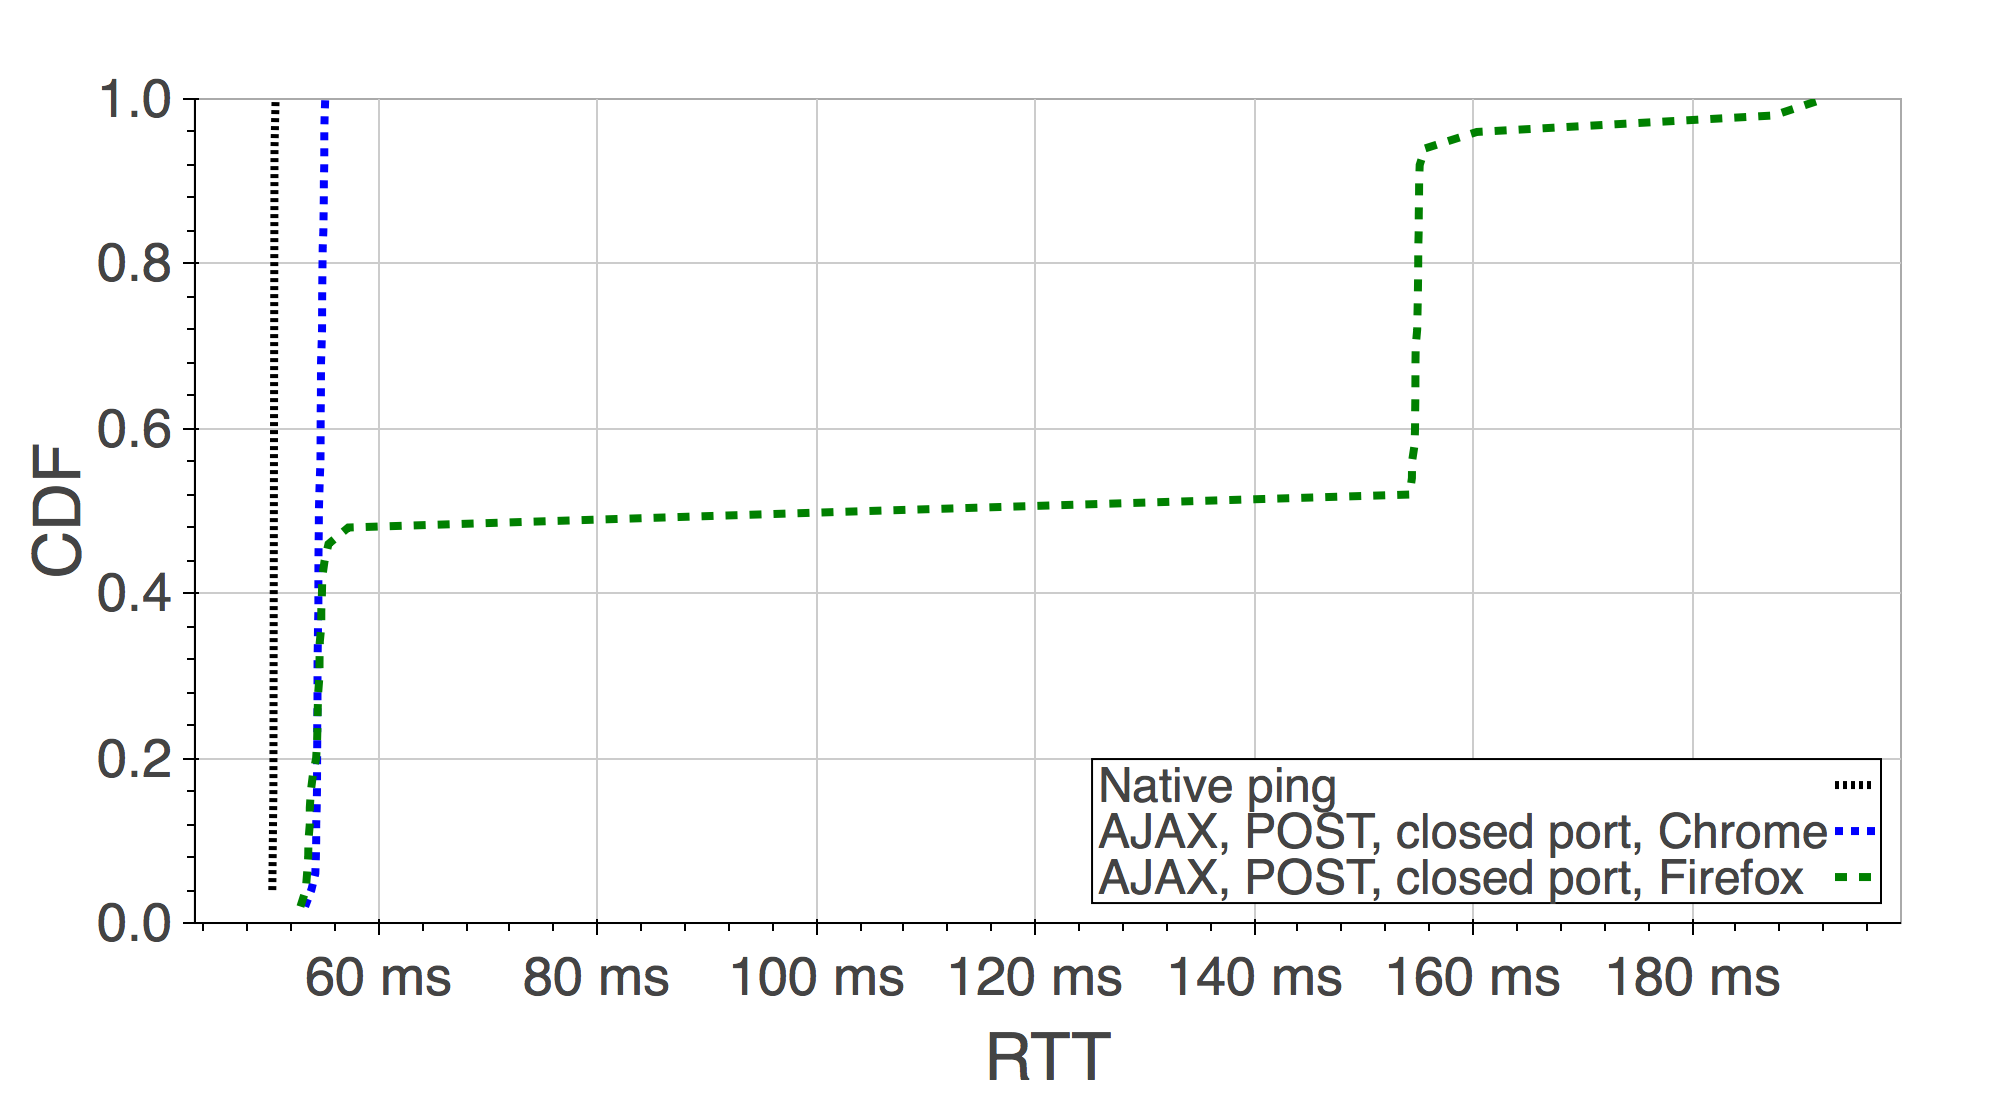
\includegraphics[width=\columnwidth]{figures/inet-comp-chrome-ff}
%\caption{Comparison of delays to an Internet server on a closed port on Linux using either Chrome or Firefox.}
%\end{figure}
%
%The cooperative measurements include a WebSocket, WebRTC ping and Ajax. For Ajax, again, POST gives the shortest RTTs while GET gives the largest but POST and HEAD have less difference than in the uncooperative case. WebSocket gives the lowest delay overheads confirming the findings of Li et al.~\cite{li:imc2013}. However, while WebSocket generally performs well, there are also few very high outliers. These occur across all OS and browsers. The packet traces reveal that these outliers are not caused by delays in the browser but rather by a processing delay of up to 20~ms in the WebSocket echo server. These findings are unexpected as the used WebSocket server \textit{WS} on node.js is widely used and the possibility of such large delays is, to our knowledge, not documented. WebRTC's accuracy is not as good as WebSocket's but unless WebSocket, WebRTC has no high outliers which makes it reliable for delay measurements. 
%
%\begin{figure}[h]
%\label{fig:inet_coop}
%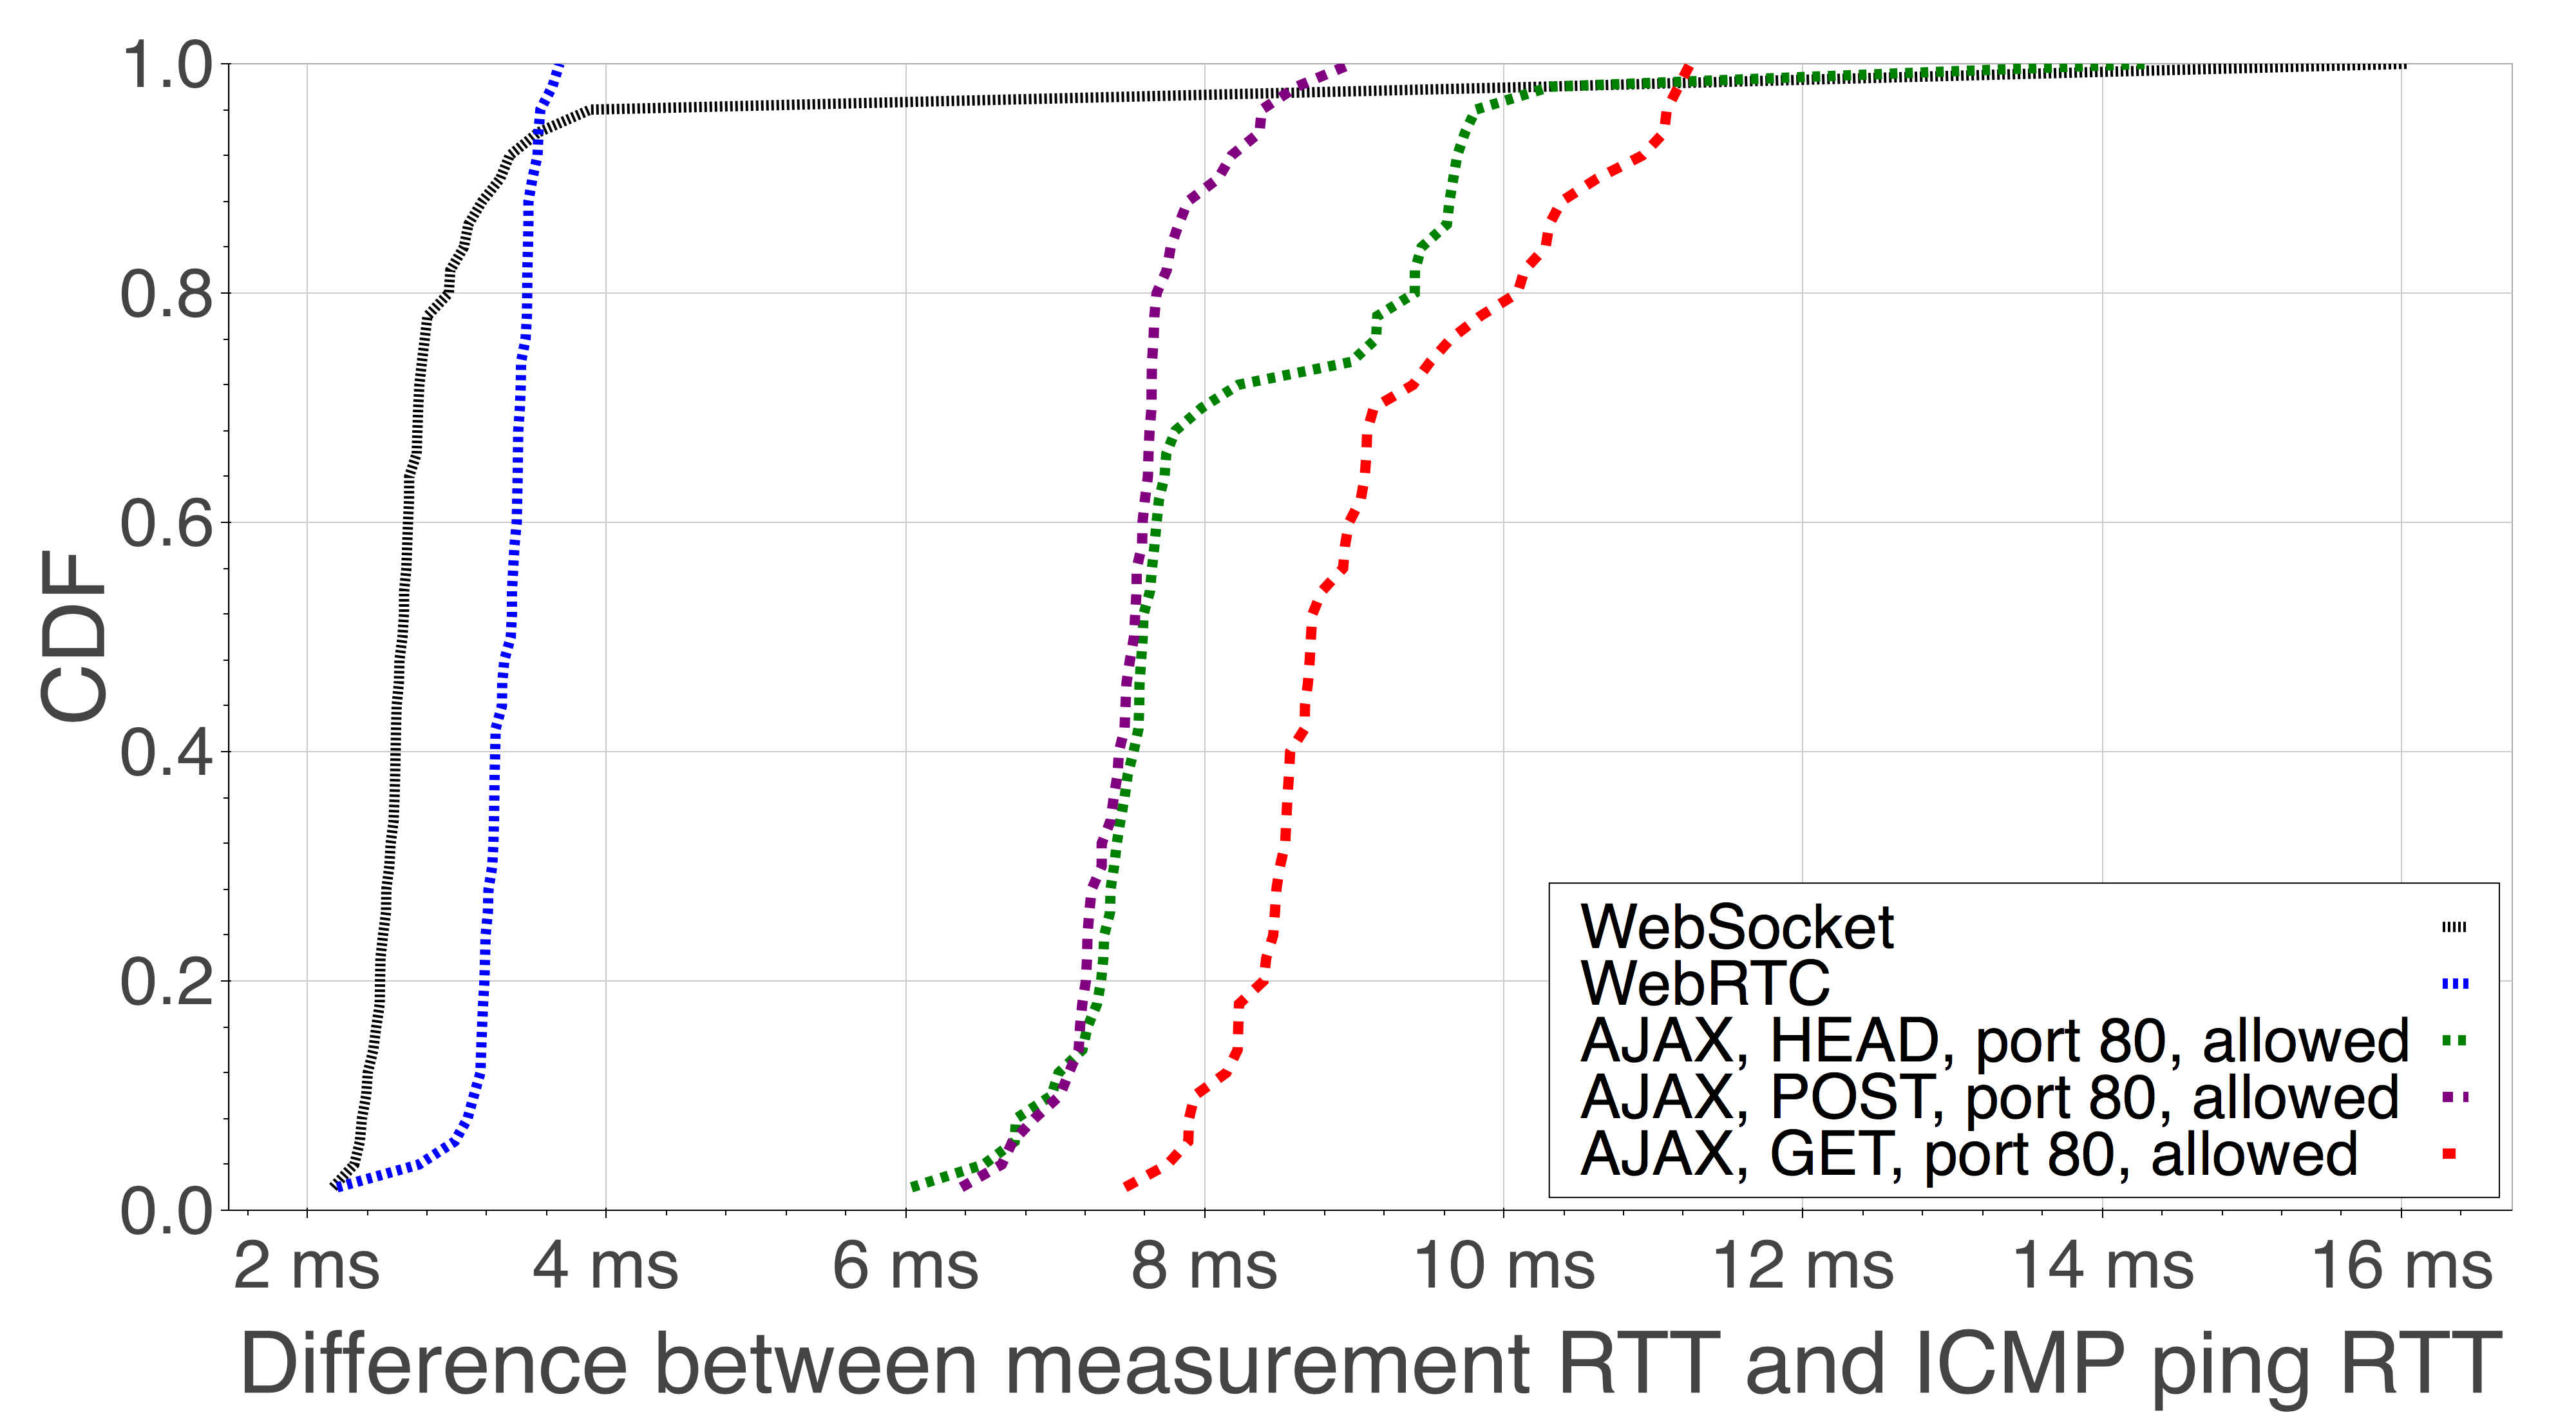
\includegraphics[width=\columnwidth]{figures/inet-coop}
%\caption{Comparison of AJAX delay overheads to a cooperating server in the Internet using either GET, HEAD or POST on Mac using Chrome.}
%\end{figure}
%
%When comparing cooperative and uncooperative approaches as well as native ping (\autoref{fig:inet_comp}), WebSocket clearly performs best out of all browser based methods
%%\footnote{Excluding Ajax to a closed port as this is generally not feasible for servers in the Internet} 
%and cooperative Ajax requests perform worst. Native ping reports significantly lower RTTs than any of the browser-based methods, however, it seems like nonetheless, web-based delay measurement approaches are promising for Internet servers as the ratio between the delays of native ping and WebSocket is low. \todo[inline]{Add number here for the ratio?}
%
%\begin{figure}[h]
%\label{fig:inet_comp}
%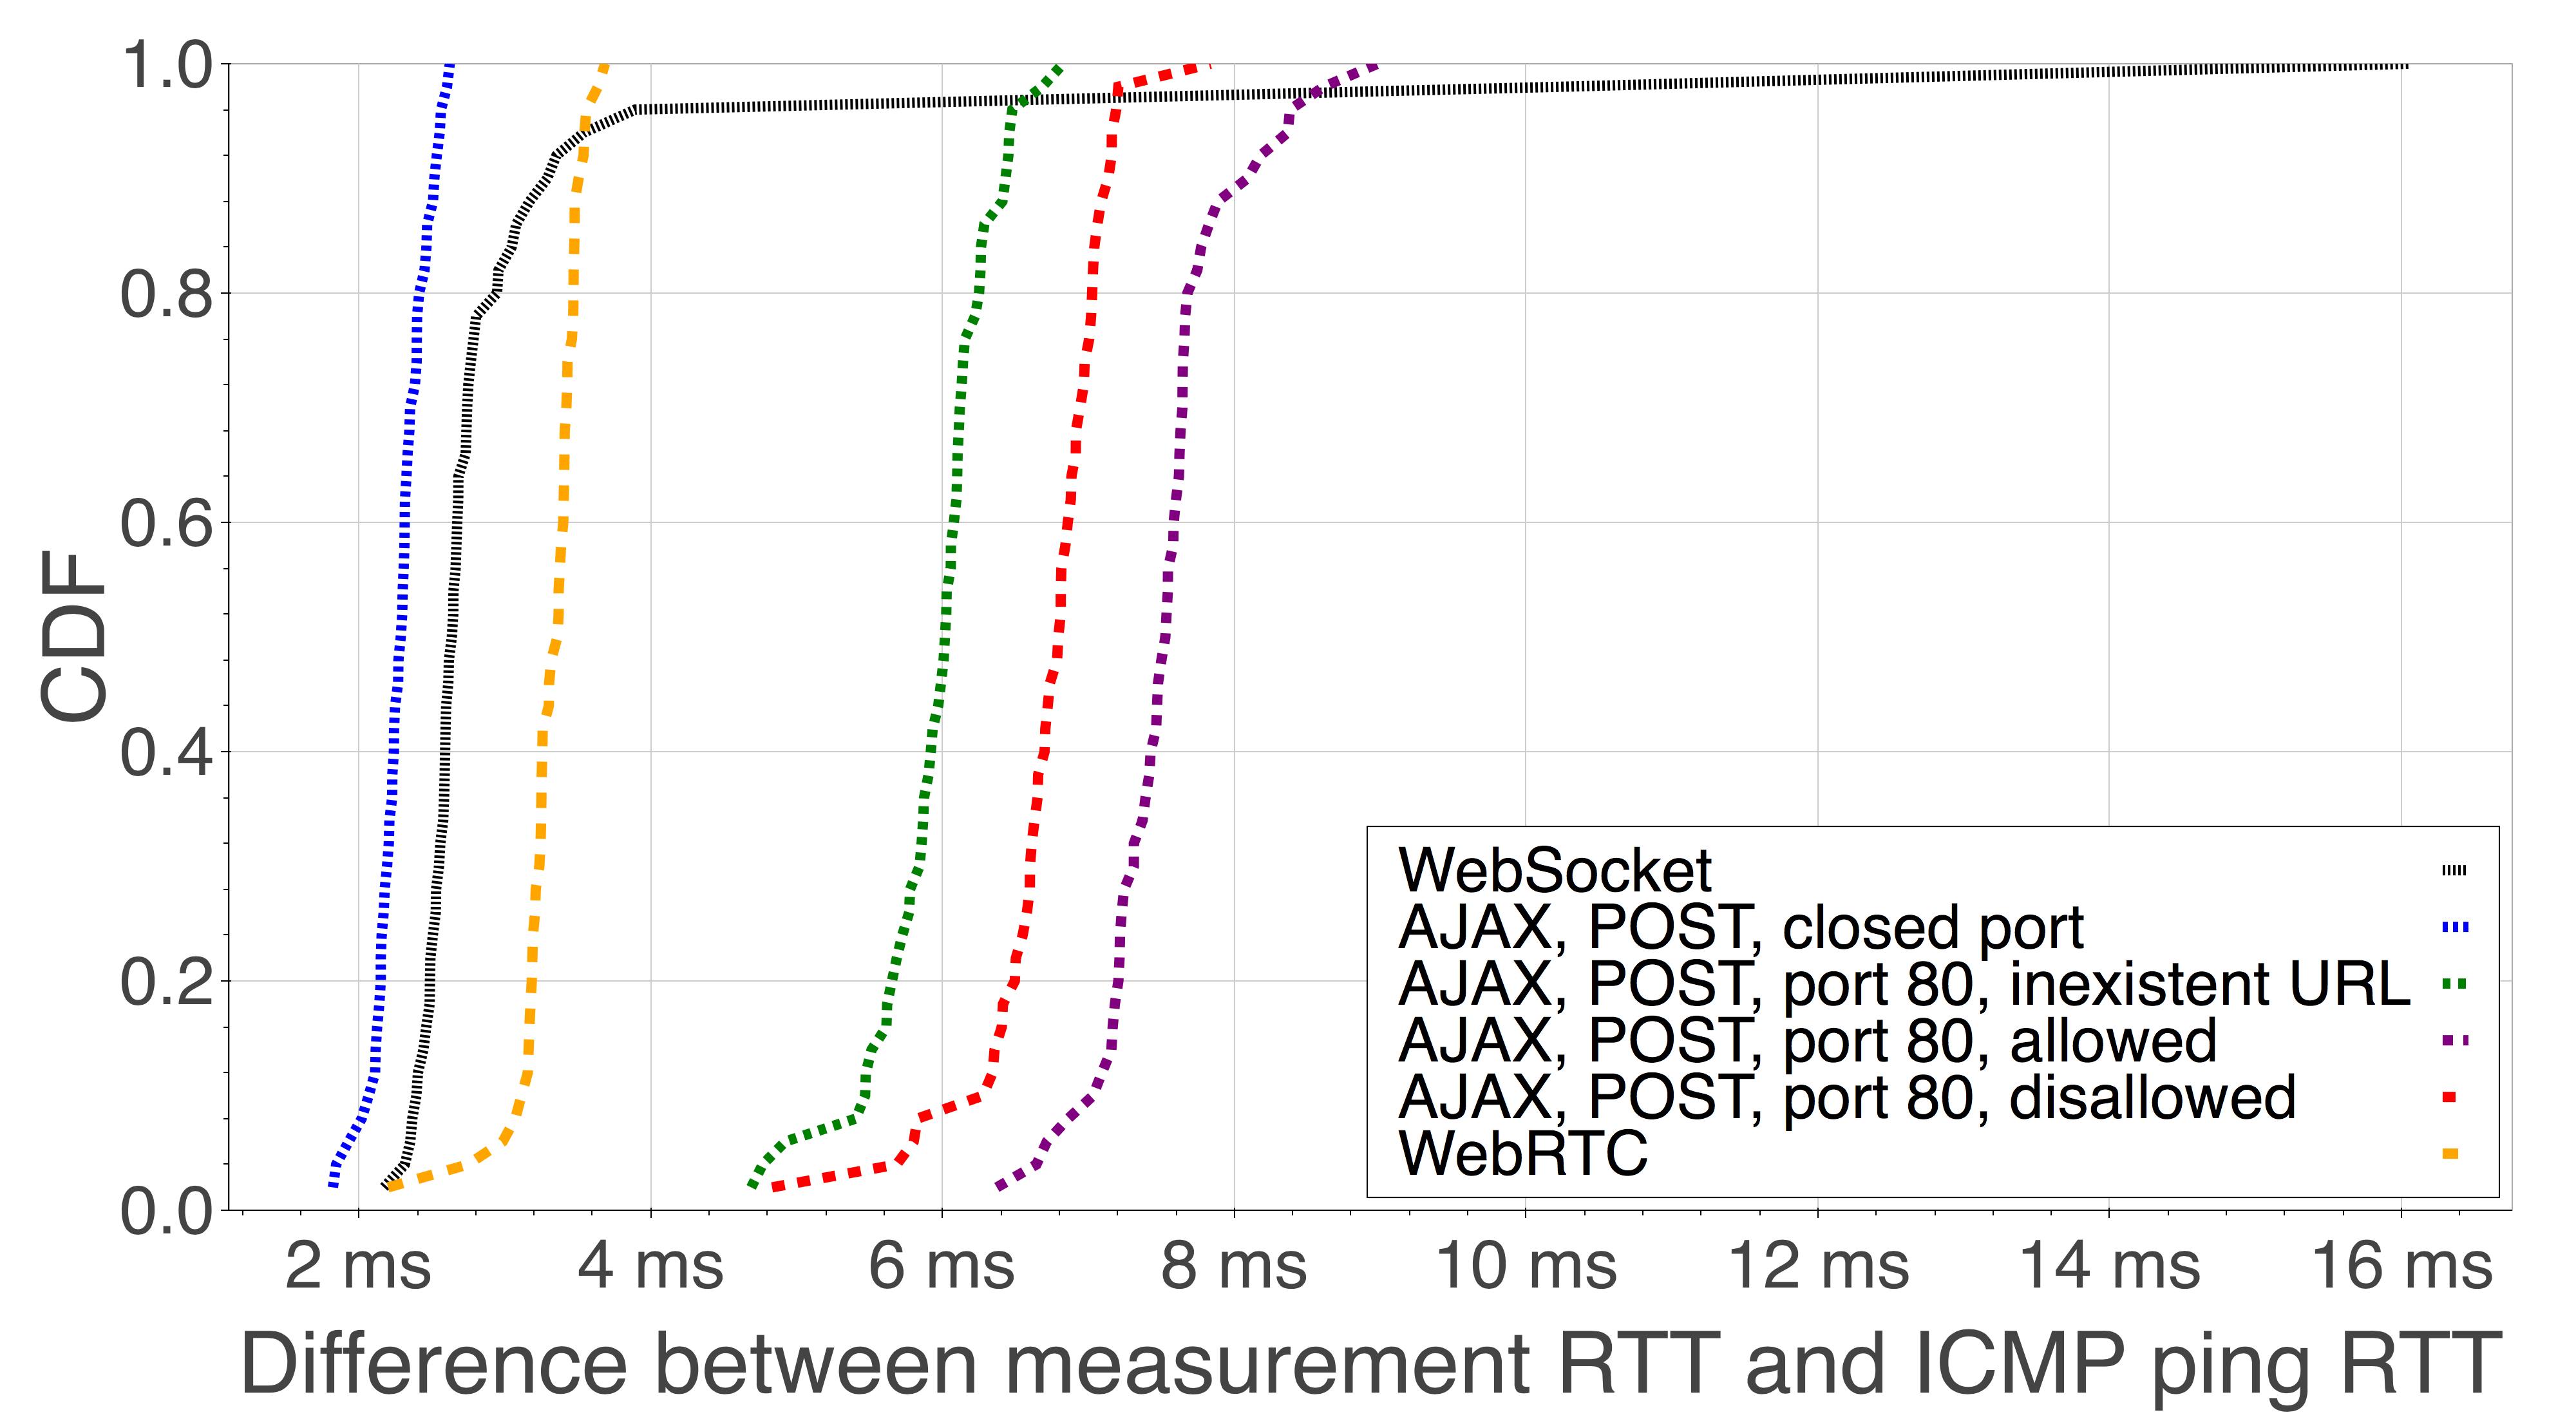
\includegraphics[width=\columnwidth]{figures/inet-comp}
%\caption{Comparison of cooperative and non-cooperative delay measurement methods as well as an ICMP ping to an Internet server on Mac using Chrome.}
%\end{figure}
%
%\section{Local delays}
%\label{sec:local}
%
%%Before the introduction of \texttt{window.performance.now} it was not feasible to measure delays within the home network because latencies are very low and the only previously available timing methods \texttt{Date.now} only offered millisecond accuracy with a granularity often higher than 1~ms \cite{li:imc2013}. It is not trivial to discover a home router's private IP address from JavaScript running on a web page. However, when a client is trying to establish a WebRTC connection to any peer, it will discover it's own private IP address, e.g.~192.168.0.107. Most home routers are configured to use the first available address within their subnet, which would be 192.168.0.1 in our example. This method enables measurement code in Web Browsers to discover their routers' private IPv4 address. 
%
%%For the local delays we compare \begin{enumerate*}[label=\alph*)]
%%\item requests to the router's web interface on port 80, requesting the index page
%%\item requests to the router's web interface on port 80 but requesting an inexistent URL
%%\item requests to a closed port on the router.
%%\end{enumerate*}
%
%\autoref{fig:router_comp} shows that when comparing all measurement methods, Ajax requests to a closed port on the router clearly gives the lowest overhead. However, this method is not available for Windows as we determined in \autoref{sec:servers}. Requesting inexistent pages has a lower latency than requesting valid ones. The packet traces show that the reason is a large processing overhead by the router for existing pages while for invalid ones, the overhead is significantly smaller.
%
%On Chrome, for requests to closed ports POST shows the lowest delay overhead, while for measurements to port 80, HEAD had the best performance. 
%\begin{figure}[h]
%\label{fig:router_comp}
%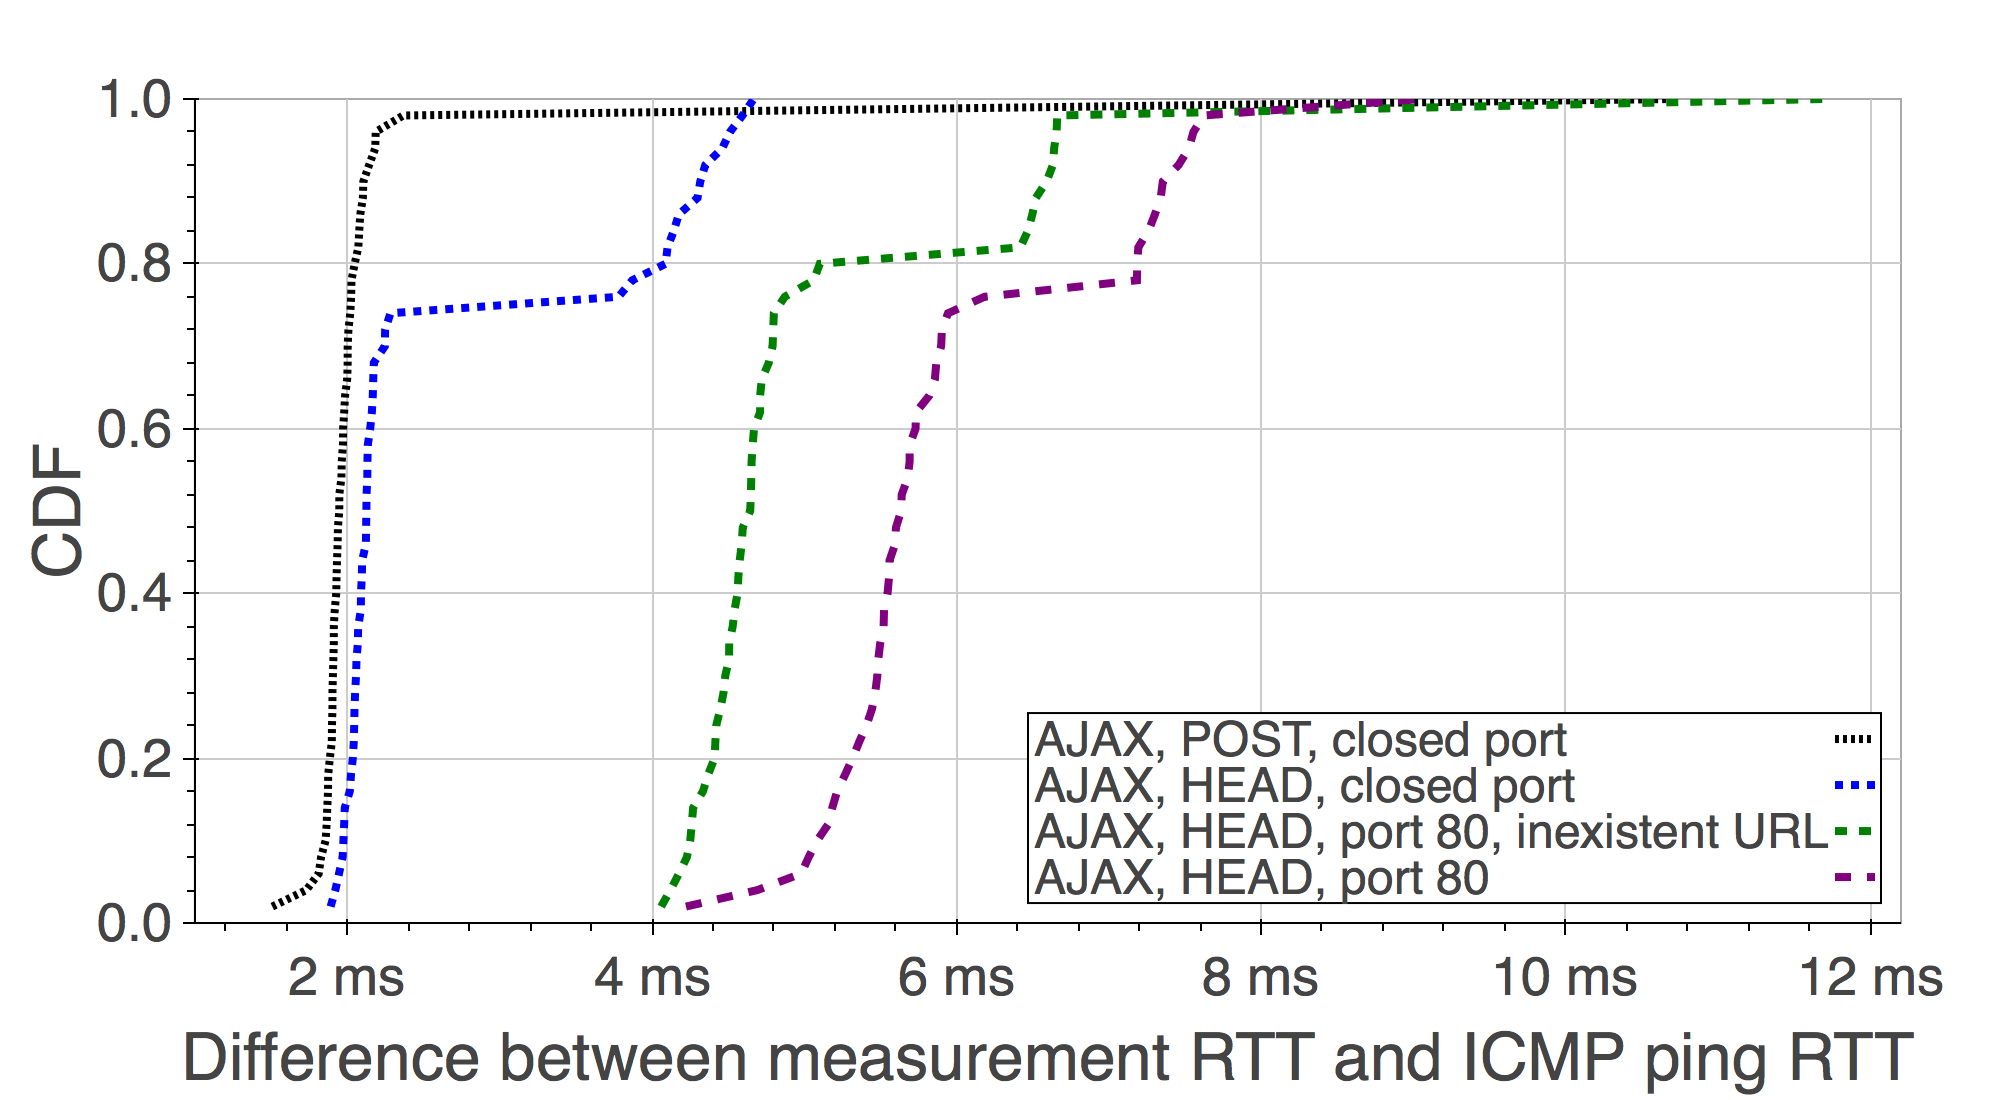
\includegraphics[width=\columnwidth]{figures/router-comp}
%\caption{Comparison of delay overheads to a home router on Mac using Chrome.}
%\end{figure}
%
%%However, the method of sending AJAX requests to closed ports only works well from an OS X or Linux host. Windows does not immediately report \textit{connection refused} to an application upon receiving a RST packet but instead retries several times before quitting the connection attempt \cite{microsoft_tcp_retries} (\autoref{fig:router_comp_mac_win}). 
%
%%\begin{figure}[h]
%%\includegraphics[width=\columnwidth]{figures/router-comp-mac-win}
%%\caption{Comparison of delays to a home router on a closed port using Chrome on both OS X and Windows}
%%\label{fig:router_comp_mac_win}
%%\end{figure}
%
%It is highly surprising that on both Chrome and Firefox there is a difference depending on whether HEAD, GET or POST are used to a closed port (\autoref{fig:router_comp-chrome-ff}) as the browser's connection attempt is rejected immediately by the router before HTTP gets involved. This proves that both Chrome and Firefox do not internally treat different HTTP methods in the same way. Firefox treats GET and HEAD in the same way and apparently handles POST with higher priority while Chrome handles all three differently. 
%
%\begin{figure}[h]
%\label{fig:router_comp-chrome-ff}
%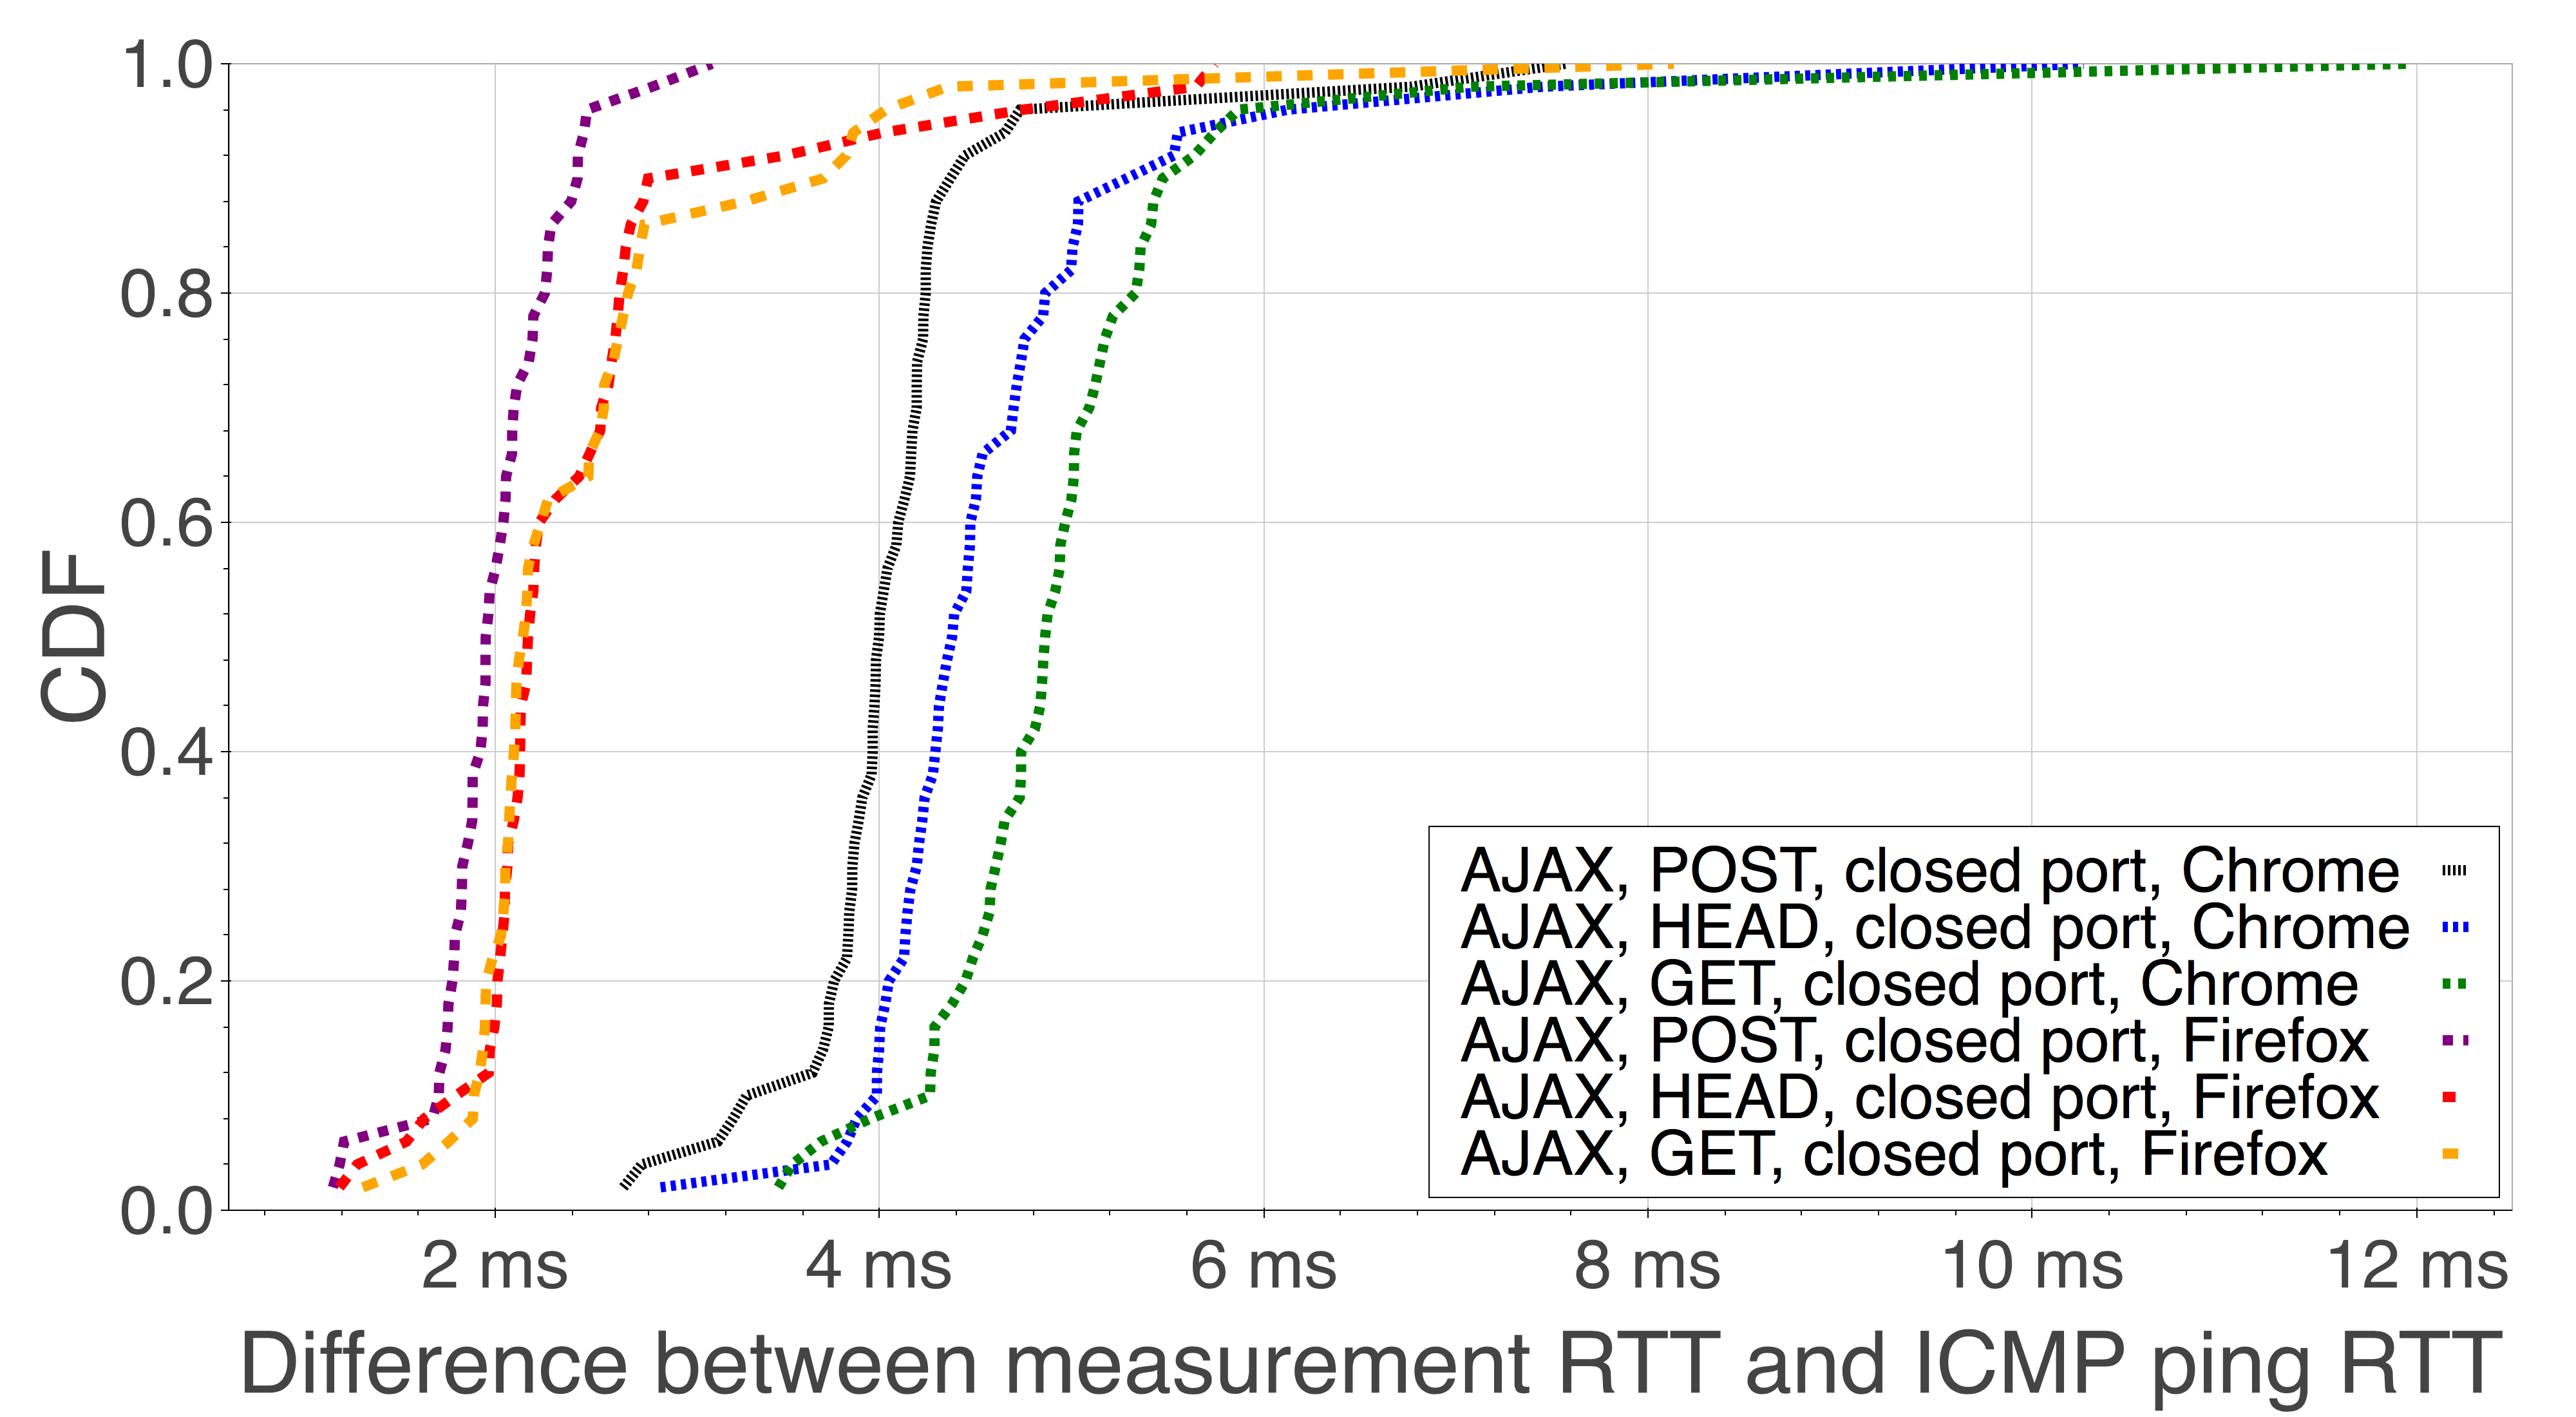
\includegraphics[width=\columnwidth]{figures/router-comp-chrome-ff}
%\caption{Comparison of delay overheads to a home router on Linux using Chrome or Firefox.}
%\end{figure}
%
%%\section{Local delays: Between devices}
%%\label{sec:local-devices}
%
%%We assume that it is useful to measure RTTs between various user devices within a household such as laptops, tablets, smartphones etc.~for the purpose of home network troubleshooting. In this case, WebRTC is promising because it is enabled in an increasing number of browsers and is capable of establishing peer-to-peer connections within a household. Because WebRTC retrieves a device's and its peer's IP address, for future work it is also possible to use Ajax requests to closed ports in similar way as performed for the home router in \S\ref{sec:router}. 
%In the case of performing delay measurements to a peer in the same network over WebRTC, our results indicate that even though the Data Channel adds several layers of encapsulation (see \autoref{subsec:webrtc}), it enables stable delay measurements and does not suffer from large outliers (\autoref{fig:router_comp_chrome_ff}). Firefox's WebRTC implementation introduces less overhead than Chrome's. \todo[inline]{Add more?} 
%
%%\begin{figure}[h]
%%\includegraphics[width=\columnwidth]{figures/other-machine-comp}
%%\caption{Comparison of delay measurements between two home devices using WebRTC and ICMP ping on Mac using Chrome}
%%\label{fig:router_comp}
%%\end{figure}
%\begin{figure}[h]
%\label{fig:router_comp_chrome_ff}
%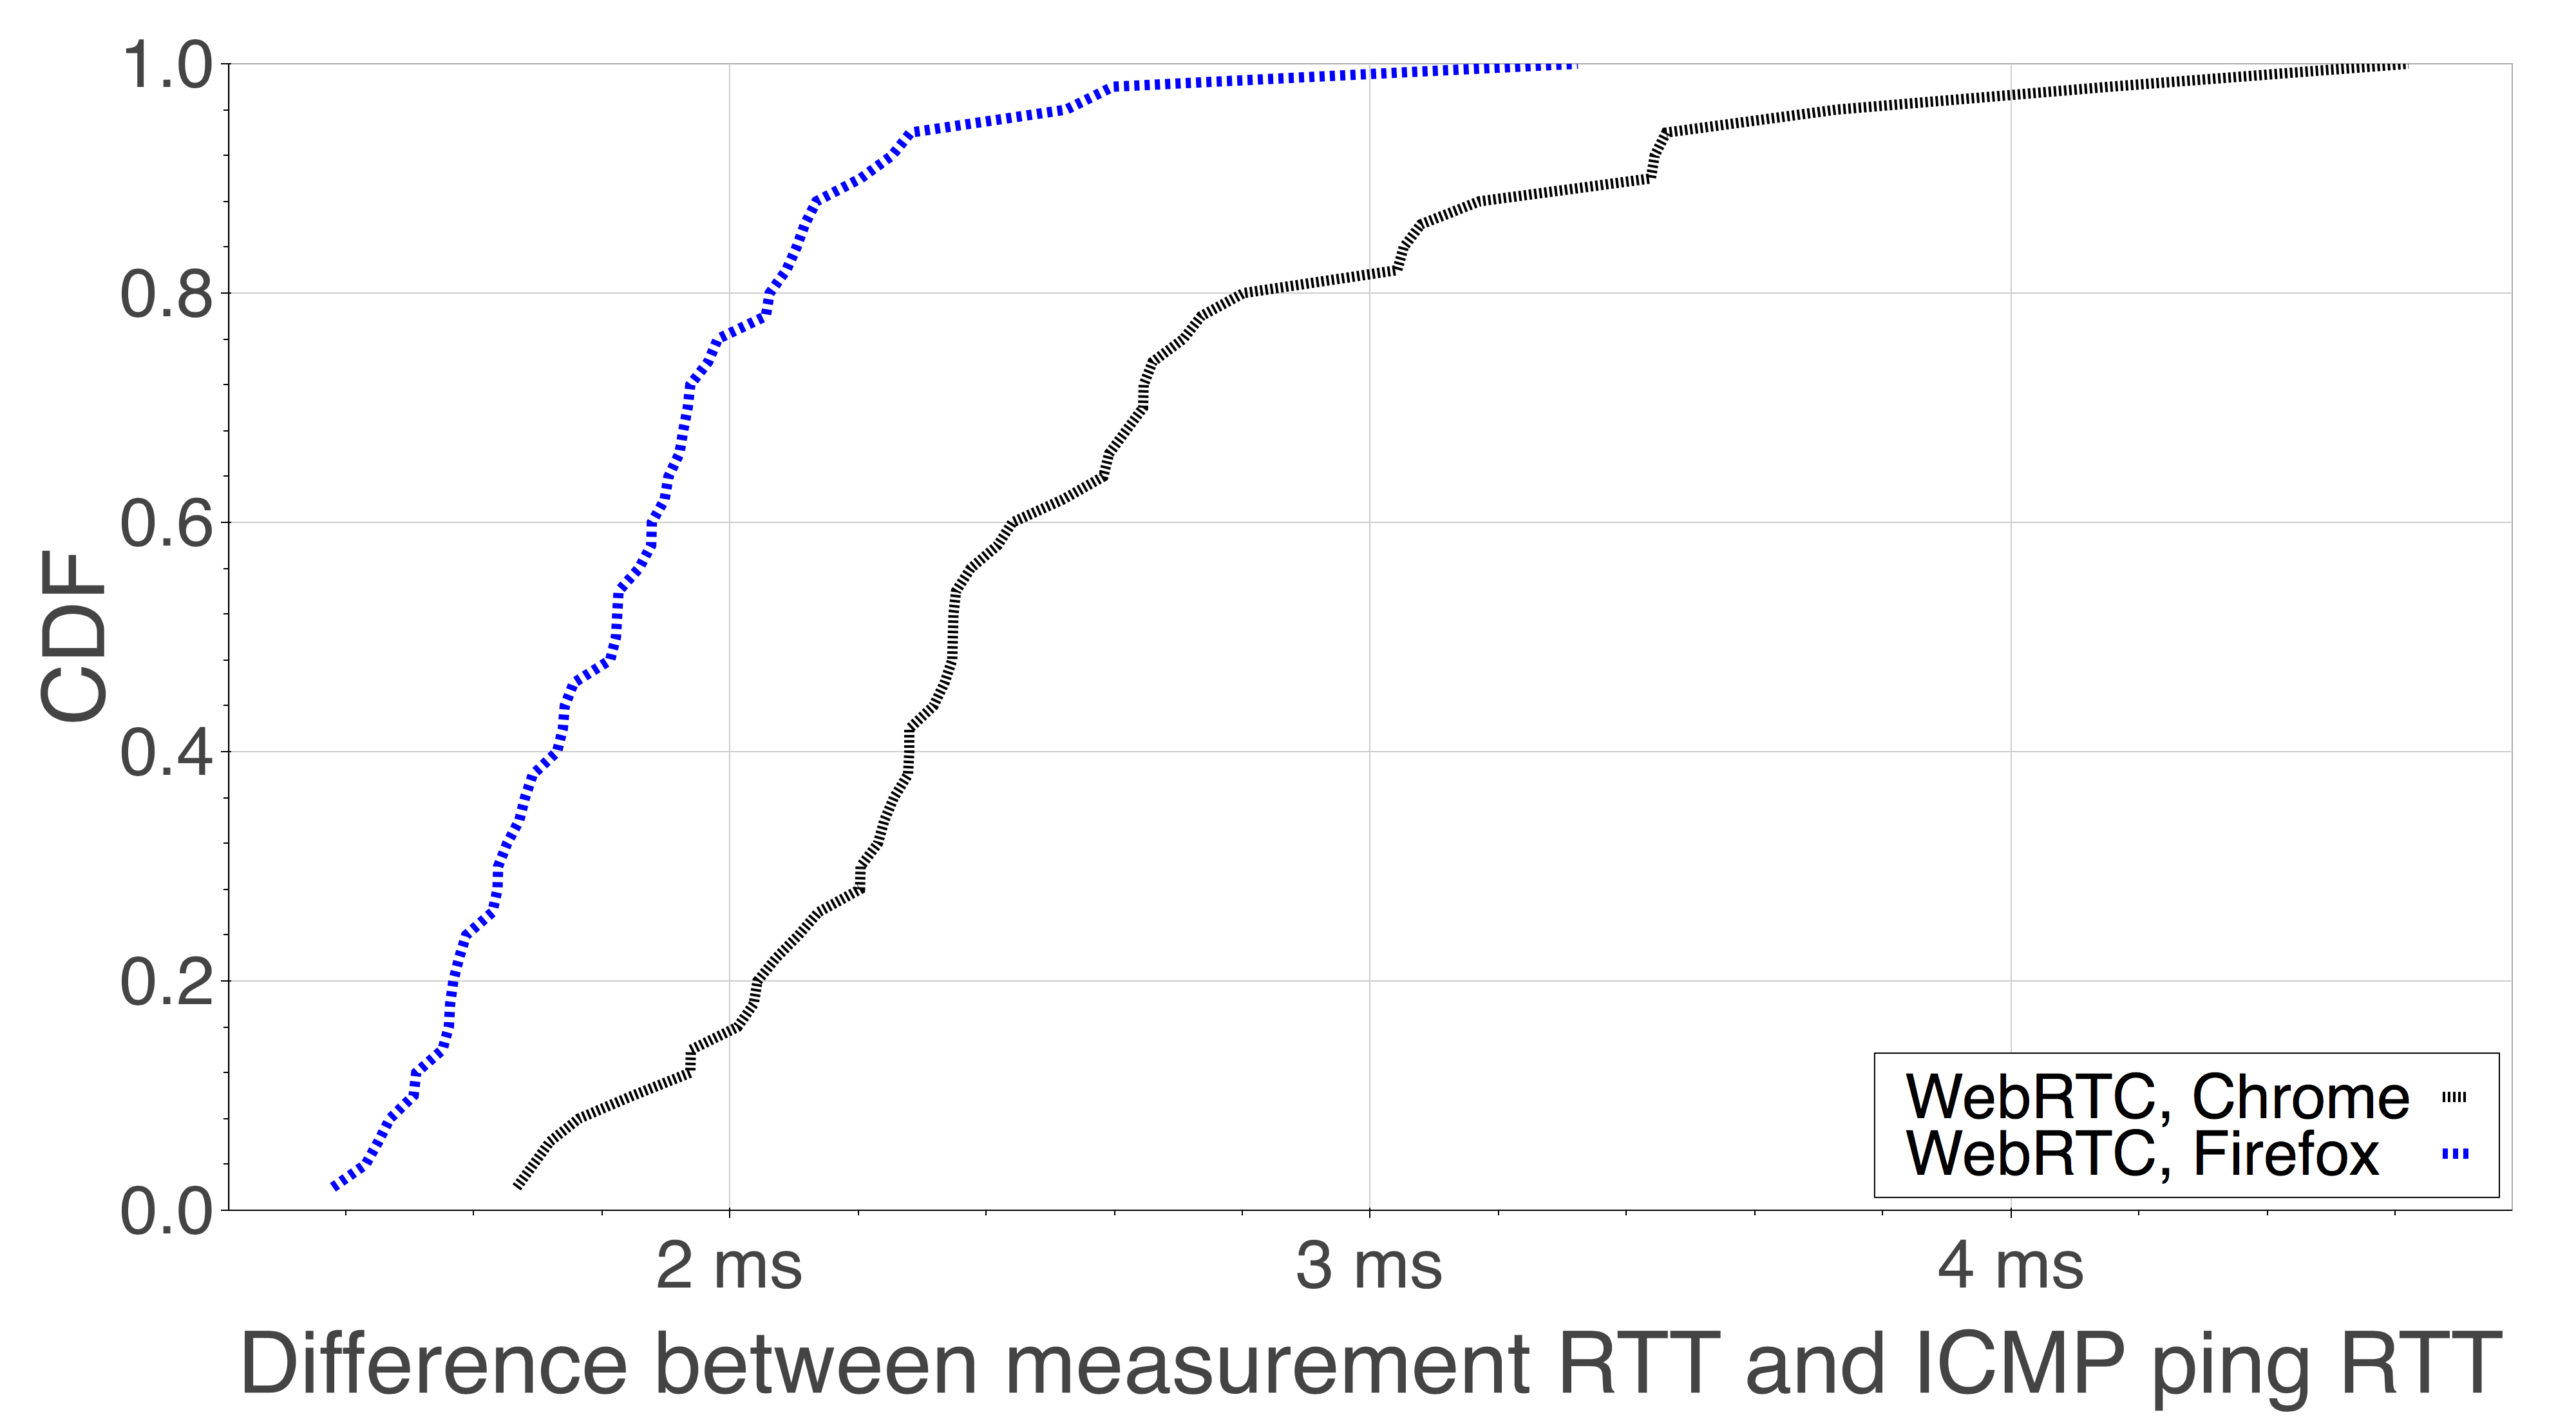
\includegraphics[width=\columnwidth]{figures/other-machine-comp-chrome-ff}
%\caption{Comparison of delay overheads between two home devices using WebRTC on Mac using Chrome or Firefox.}
%\end{figure}
%
%\section{Influence of load}
%
%Our results show that different operating systems do not have an influence on the behavior with or without load when using the same browser. However, we concluded that Firefox is influenced by passive browsing (\autoref{fig:inet_comp_load_chrome_ff}). The difference does not depend on the measurement method used. Chrome, on the contrary, does not display different behavior when exposed to load. This might be caused by the multi-process architecture of Google Chrome \cite{chrome_multi-process_2008} where each web page runs in an independent process while in Firefox, currently, there is one process for all web pages and for the browser UI \cite{firefox_multiprocess_2016}. Generally, our experiment shows that load can have a severe impact on the delay overheads for browser based measurements, as related work (\cite{Sommers07,holterbach:2015}) has shown for other measurement platforms at the Internet's edge.
%\begin{figure}[h]
%\label{fig:inet_comp_load_chrome_ff}
%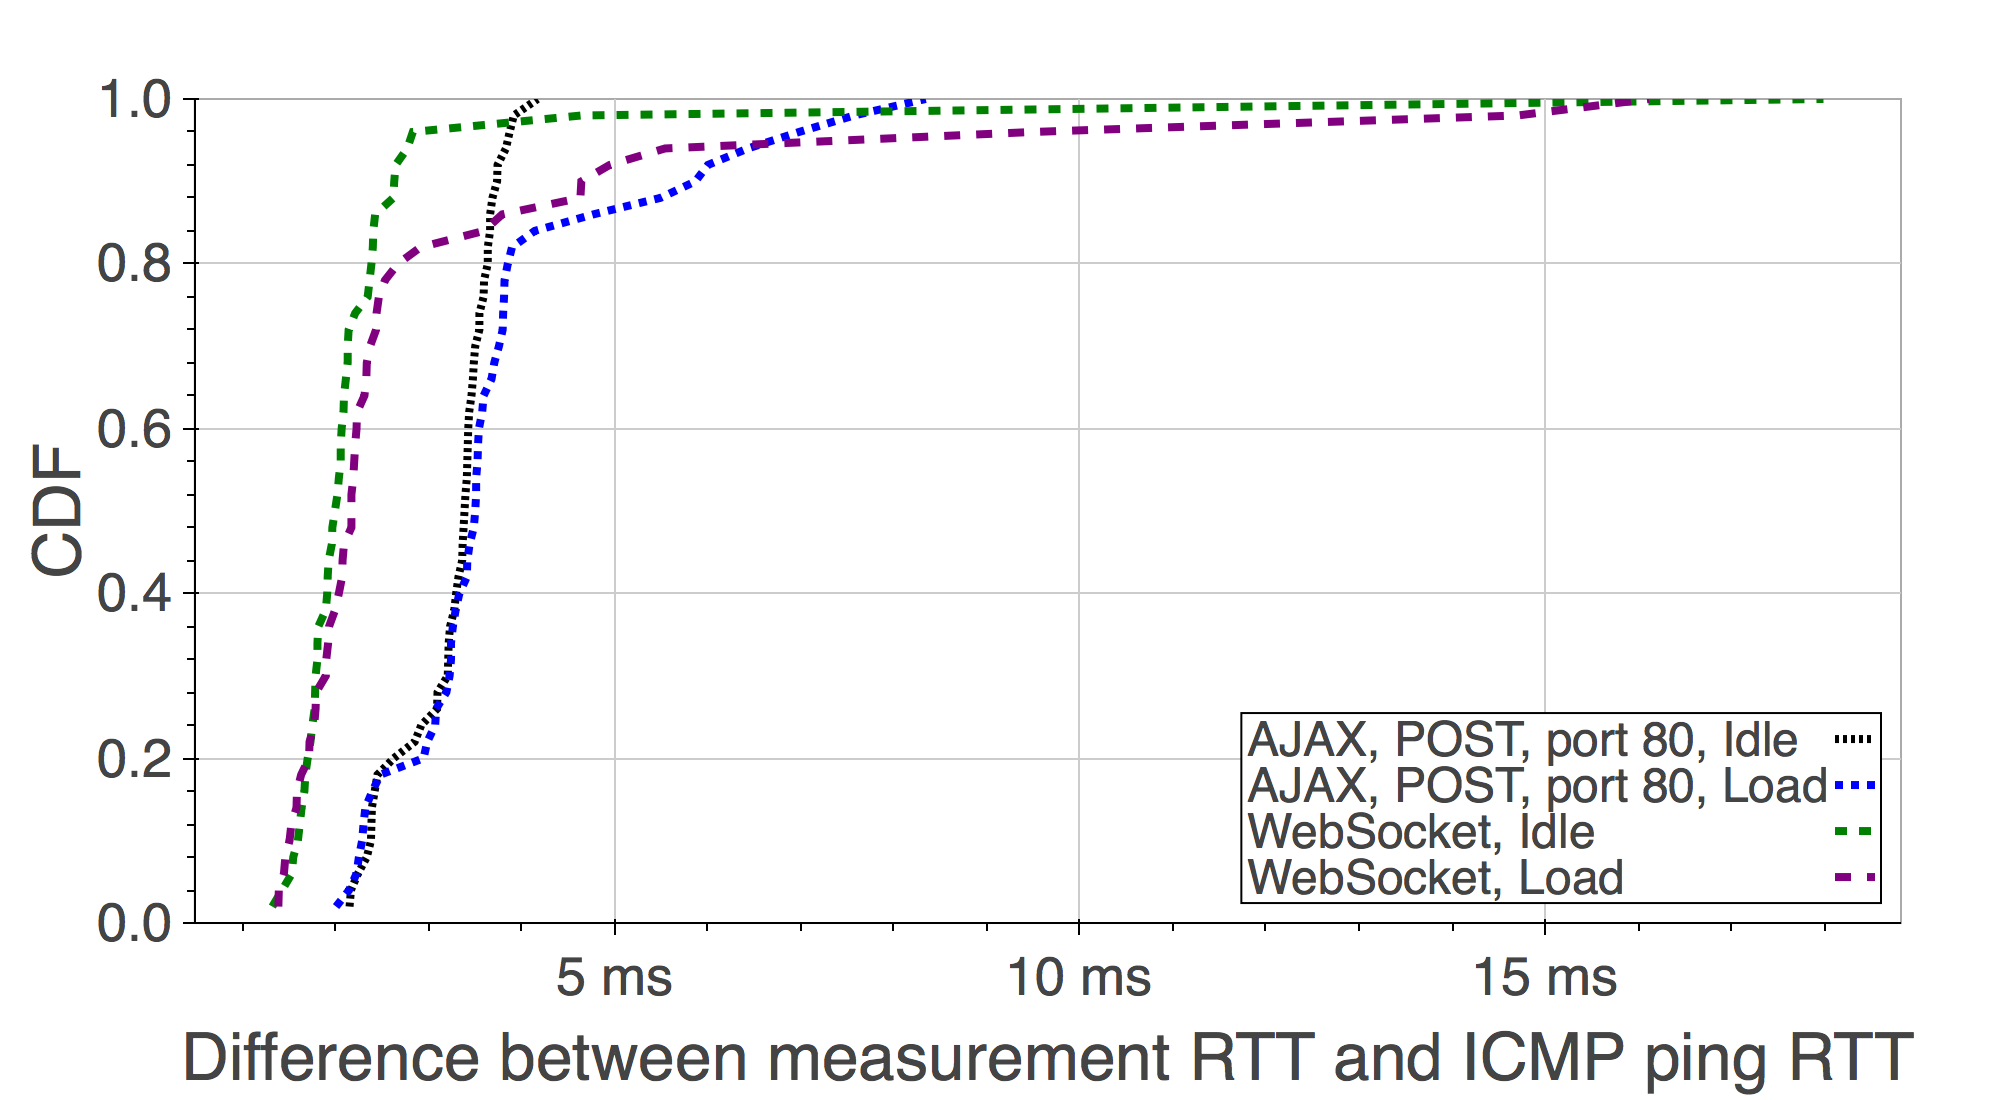
\includegraphics[width=\columnwidth]{figures/inet-comp-load-ff}
%\caption{Comparison of delay overheads to an Internet server on Windows using Firefox when being idle or under load.}
%\end{figure}

\section{Related Work}

Our work is motivated by the need to measure from within the Internet's edge. A number of previous work have recognized the need for measurement platforms to better cover the Internet's edge, starting from SatelliteLab~\cite{satellitelab}, which aimed at extending PlanetLab to include nodes in edge networks. Since then, the networking research and operations communities have deployed a number of systems and platforms to launch measurements from the Internet's edge. Some groups distribute hardware that users then connect to edge networks---popular examples are RIPE Atlas~\cite{ripe-atlas} and BISmark~\cite{bismark}; others rely on software that users install directly on their end systems, for example, the Fathom Firefox extension~\cite{fathom} and the Dasu BitTorrent plugin~\cite{dasu}. Many of these systems use M-Lab~\cite{m-lab} servers as target because they are well-provisioned and connected to multiple locations in the Internet. 

Running measurement scripts directly from browsers as we evaluate in this paper eliminates the need to deploy measurement hardware or install measurement software. Hence, a number of tools for users to test their Internet performance take this approach, for instance, Ookla's speedtest~\cite{speed-test}, NDT~\cite{www-ndt}, and Netlyzr~\cite{kwnp10netalyzr}. The methods we present and evaluate in this paper are an asset to these tools and others that aim at measuring the performance from within edge networks. 

One issue of making measurements from browsers is the loss in measurement accuracy (as our results in \S\ref{sec:servers}--\ref{sec:local} show). Prior work has warned about inaccuracies when running measurements in PlanetLab~\cite{Sommers07} and RIPE Atlas~\cite{holterbach:2015}. Most similar to ours is the study by Li et al.~\cite{li:imc2013}, which also studies the accuracy of delay measurements from browsers. We reappraise their results in \S\ref{sec:servers} in view of today's web technologies. In particular, we remove the analysis of Flash and Java, which are no longer enabled by default, and add the analysis of WebRTC. We also use the more recent high-resolution time API, which is available today. We introduce new methods for performing measurements to cooperative and non-cooperative targets.  In addition to testing Internet delays, we also test the more challenging scenario of local delays (in \S\ref{sec:local}), where measured values are smaller than the overheads browsers typically introduce.

\section{Conclusion}

In the first part, we explored the potential of using the web browser as a vantage point to measure RTTs from edge networks. 
%We perform controlled experiments from popular browsers and operating systems to study the overhead that browsers introduce when measuring RTTs in different scenarios. We compare several methods to measure RTTs---AJAX (HEAD, GET, POST), WebSocket, and WebRTC DataChannel. 
We first consider the case when the target is a cooperating server connected to the Internet. Our results confirm previous findings that in most cases WebSocket have the lowest overhead. WebSocket, however, sometimes introduce significant overhead (of 20~ms) making it an unreliable method to measure RTTs. Our experiments with WebRTC presented overheads that are only slightly higher than that of WebSocket but very consistent; making it the best choice for measuring Internet delays to cooperating targets. Then,
we considered the case when measuring Internet delays to non-cooperating targets. We saw that opening an AJAX connection to a closed port introduces the lowest overhead, but it is not reliable on Firefox and on Windows. An alternative is to use AJAX to an inexistent URL.  Finally, we considered cases where targets are in the local network. Both WebRTC between devices and AJAX to a closed port work well, but they introduce overheads around 2--4~ms. This is particularly challenging as the delays within local networks are in the same order as the measurement overhead browsers introduce. 

%\begin{table*}[t]
%\label{comparison}
%\centering
%\begin{tabular}{ll|ll|ll|ll}
%\noalign{\hrule height 1pt}
%\multirow{2}{*}{OS} & \multirow{2}{*}{Browser} & \multicolumn{2}{l|}{Router} & \multicolumn{2}{l|}{Other machine} & \multicolumn{2}{l}{Server} \\
%%\cline{3-8}
%&& Value & Method & Value & Method & Value & Method\\
%\noalign{\hrule}
%\multirow{2}{*}{OS X} & Chrome & 1.9 [1.8, 2.2] &Ajax Post, closed & 2.3 [1.7, 3.6] &WebRTC & 2.3 [2.0, 2.6]& WebSocket \\
%& Firefox & 3.1 [2.9, 3.4] &Ajax Get, closed & 1.8 [1.5, 2.4]& WebRTC & 2.4 [2.0, 3.5]& WebSocket\\
%\noalign{\hrule}
%\multirow{2}{*}{Ubuntu} & Chrome & 4.0 [3.3, 4.7] &Ajax Post, closed & 2.7 [2.2, 3.1]& WebRTC & 2.8 [2.5, 4.0]& WebSocket\\
%& Firefox & 2.0 [1.4, 2.5]& Ajax Post, closed & 1.8 [1.5, 2.1]& WebRTC & 2.4 [2.1, 7.1]& WebSocket \\
%\noalign{\hrule}
%\multirow{2}{*}{Win.} & Chrome & 3.7 [2.3, 4.3]& Ajax Post, inval.~path & 2.1 [1.4, 2.5]& WebRTC & 2.1 [1.6, 4.1]& WebSocket\\
%& Firefox & 3.3 [1.6, 3.7]& Ajax Post, inval.~path & 1.7 [1.0, 2.1]& WebRTC & 2.0 [1.5, 2.8]& WebSocket\\
%\noalign{\hrule height 1pt}
%\end{tabular}
%\caption {Measurement method with least overhead in milliseconds selected for each OS and browser by median in case of no additional load in the browser. 5th and 95th percentiles in brackets}
%\end{table*}
%
%Generally impossible to achieve less than 2ms overhead, however some methods deliver results with pretty constant overhead. 

\chapter{Easy home network troubleshooting}
\label{chap:troubleshooting}

\section{Introduction}

\cleardoublepage
\phantomsection
\addcontentsline{toc}{chapter}{Bibliography}

%\printbibliography
\bibliographystyle{abbrv}
\bibliography{thesis}

%\cleardoublepage
%\phantomsection
%\addcontentsline{toc}{chapter}{List of Figures}
%\listoffigures

\end{document}  



